% IOP Publishing journal manuscript (English submission version).
% Based on the supervisor's English draft (docs/导师英文稿.pdf) and updated with
% the todo1102 experiments (sealed hold-out, leave-cluster-out audit,
% noise-augmented training, random-kernel noise tests, 36-D feature screen,
% ONNX/int8 export). Figures are the English versions in figures_en/.
% Build: xelatex (or pdflatex) twice; see README.md.
\documentclass{iopjournal}

\usepackage{iftex}
\ifPDFTeX
  \usepackage[T1]{fontenc}
  \usepackage[utf8]{inputenc}
\fi
\usepackage{amsmath,amssymb,bm}
\usepackage{booktabs}
\usepackage{array}
\usepackage{tabularx}
\usepackage{multirow}
\usepackage{cite}

\setlength{\headheight}{15pt}
\newcolumntype{Y}{>{\raggedright\arraybackslash}X}
\newcommand{\pmv}[2]{$#1\pm#2$}

\begin{document}

\articletype{Paper}

\title{Few-shot classification of lithium-ion battery charging power curves with a time-series foundation model}

\author{Zhuotao Qian$^{1,*}$ and Chenghua Feng$^1$}

\affil{$^1$Hangzhou Dianzi University Information Engineering School, Hangzhou 311305, Zhejiang, People's Republic of China}

\affil{$^*$Author to whom any correspondence should be addressed.}

\email{20221009@hdu.edu.cn (Z.Q.); 239500314@hziee.edu.cn (C.F.)}

\keywords{lithium-ion battery, charging power curve, time-series foundation model, few-shot learning, anomaly classification, mask-aware pooling, stacked ensemble, noise-augmented training}

\begin{abstract}
Charging power curves from electric bicycles contain information associated with charger faults and battery anomalies, but verified fault labels are expensive to obtain and the records vary in length from 18 to 816 samples. A general time-series foundation model transfers poorly to such curves, whereas a task-specific network becomes unstable when only a small labeled subset is available. We develop a three-class method that combines a frozen time-series foundation model with raw-scale dynamics features and a masked temporal convolutional network (TCN). Mask-aware patch pooling prevents padded patches from entering the pooled MOMENT representation and raises the test Macro-F1 of a frozen linear probe from 69.46\% to 77.41\%. A first-difference stream restores local changes that patch encoding tends to smooth, increasing the single-branch validation Macro-F1 from 83.91\% to 93.57\% with 40\% of the training labels. A 60-dimensional dynamics branch retains absolute power levels, and five-fold cross-fitted probability stacking combines the three branches. On 35,099 operational charging records under a unified fixed-hyperparameter protocol, the complete model reaches validation Macro-F1 scores of $89.15\pm0.98\%$, $93.85\pm0.43\%$ and $95.13\pm0.19\%$ with 1\%, 5\% and 10\% of the training labels, exceeding the masked TCN by 27.24 percentage points at 1\%. In the cross-fitted configuration with a joint dual-stream probability block, it reaches $98.09\pm0.23\%$ with 40\% of the labels, with 98.23\% battery-anomaly recall at a 0.67\% false-positive rate, and a retrained model scores $97.76\pm0.10\%$ on a sealed hold-out set of 3,677 records drawn by identifier cluster. Pretraining contributes 6.00--18.81 percentage points to the dual-stream branch. Training all branches with noisy copies raises the 40\%-label Macro-F1 under Gaussian noise of 0.5\% of the signal root mean square from 64.72\% to 97.47\% without lowering clean accuracy, but stronger noise remains a failure point. A random-kernel classifier is more accurate below 20\% labels, which bounds the claims of this work.
\end{abstract}

\section{Introduction}\label{sec:intro}

Lithium-ion batteries power most electric bicycles used for short urban trips. During charging, an internal short circuit, cell mismatch, abnormal charger output, or a failed protection circuit can lead to overheating and, in severe cases, thermal runaway~\cite{feng2018}. Detecting abnormal behavior during charging is therefore an important part of fire-risk reduction.

Many battery fault-diagnosis systems use cell voltage, temperature, current, and other signals collected by a battery management system (BMS)~\cite{zhang2023,hu2020}. This information supports accurate diagnosis but is unavailable from many electric-bicycle batteries because models differ widely and external communication interfaces are often absent. A charging facility can usually collect only a single power sequence. If normal charging, battery anomalies, and charger faults can be distinguished from this sequence, the facility can provide non-intrusive monitoring without modifying the battery. Related studies have demonstrated fault identification for electric-vehicle charging equipment and anomaly detection from charging data~\cite{park2022,duan2024,xu2025,sun2025}, but electric-bicycle charging curves have received less attention.

This task presents three practical difficulties. First, record length varies from 18 to 816 samples. Batches require extensive right padding, and length itself is correlated with class. A model may consequently learn a padding shortcut instead of the power shape. Second, useful evidence occurs at different scales. Absolute power distinguishes low-power plateaus, local differences reveal spikes and steps, and the full curve describes the transition from a constant-power region to decay. Third, fault labels require manual verification against maintenance records and are scarce in normal operations.

Time-series classification and anomaly detection have been reviewed extensively~\cite{chen2021,xu2026,fawaz2019,middlehurst2024}. Classifiers include feature-based methods~\cite{breiman2001,friedman2001,cortes1995}, task-specific neural networks such as temporal convolutional networks (TCNs)~\cite{bai2018}, Transformer variants~\cite{liu2026,yang2026,jiang2026} and TimesNet~\cite{wu2023}, and random-kernel transforms such as ROCKET, MiniRocket, MultiRocket, and Hydra~\cite{dempster2020,dempster2021,tan2022,dempster2023}. Transfer learning and self-supervised representation learning can reduce label requirements~\cite{wang2026,yue2022}. More recently, foundation models such as MOMENT, TimesFM, Chronos, Moirai, and Time-MoE have been pretrained on large, heterogeneous collections of time series~\cite{goswami2024,das2024,ansari2024,woo2024,shi2025}. Their representations have been studied in machinery diagnosis, engineering displacement prediction, and input-representation design~\cite{shao2026,zhao2026,yang2026b}.

Direct transfer is not sufficient in the present task. Freezing MOMENT-1-large and training its default classification head yields only 69.46\% test Macro-F1, compared with 95.99\% for a task-specific TCN trained on raw-scale curves. We trace this mismatch to three operations. The default head averages padded patches; patch encoding smooths short power changes; and per-series normalization removes absolute amplitude. We address each operation without updating the 341.24 million backbone parameters.

The contributions are as follows. First, mask-aware patch pooling excludes incomplete and padded patches and makes the frozen representation invariant to the padded region. Second, a first-difference stream supplies local change information to the same frozen encoder. Third, a 60-dimensional raw-scale dynamics branch restores amplitude and interpretable local statistics, and five-fold cross-fitted stacking combines the foundation-model branch, the dynamics branch, and a masked TCN. Fourth, we delimit where the method is useful. Paired ablations, same-architecture pretraining controls, and label-budget experiments separate the sources of improvement. A sealed hold-out set disjoint by identifier cluster and a leave-cluster-out audit address selection on repeatedly used validation data. Noise-augmented training, a noise-matched comparison with random-kernel classifiers, and latency and model-export measurements identify the operating conditions under which the proposed model, a lighter TCN-based model, or a random-kernel classifier should be preferred.

\section{Problem formulation and data}\label{sec:data}

\subsection{Task definition}

Let the valid power sequence for record $i$ be $\bm{x}_i=(x_{i,1},x_{i,2},\ldots,x_{i,L_i})$, where $18\le L_i\le 816$. For batching, the sequence is right-padded to $T=1024$ and paired with a binary mask $\bm{m}_i\in\{0,1\}^T$, where $m_{i,t}=1$ for a valid observation and $m_{i,t}=0$ for padding. The classifier learns
\begin{equation}
f:(\bm{x}_i,\bm{m}_i)\mapsto y_i\in\{0,1,2\},
\label{eq:task}
\end{equation}
where labels 0, 1, and 2 denote normal charging, a battery anomaly, and a charger fault, respectively. An ideal classifier is invariant to both the amount and the values of right padding.

\subsection{Dataset}\label{sec:dataset}

The data consist of operational records from an electric-bicycle charging platform. Each record contains an anonymized identifier, an operational label, and a charging power sequence. Of 46,535 original records, 11,435 carry the platform's label 5 for an invalid or incomplete record; their median length is one sample. These records were excluded under the platform's established protocol. Records shorter than 18 samples were also removed, leaving 35,099 valid sequences. The threshold of 18 was inherited from the existing experimental protocol; the data provider has not supplied an independent physical interpretation for it. Sampling intervals were not included in the source data, so this study reports sequence length only in samples and does not convert it to elapsed time. No duplicate sequences or label conflicts were found. The longest sequence contains 816 samples and is not truncated at $T=1024$. A stratified 7:1:2 split defines the training, validation, and test sets (table~\ref{tab:split}). In the first two experimental stages, every method uses the same split files; section~\ref{sec:protocol} describes the re-partitioning used for the sealed hold-out stage.

The source data contain no time stamps, site fields, device models, or batch fields. Every identifier is unique, but identifiers sharing their first six characters form 8,075 groups that we use as a proxy for deployment clusters in section~\ref{sec:holdout}.

\begin{table}[htbp]
\caption{Dataset split and class distribution.}
\label{tab:split}
\centering
\begin{tabular}{l r r r r}
\toprule
Subset & Normal (0) & Battery anomaly (1) & Charger fault (2) & Total \\
\midrule
Training & 8,480 & 7,014 & 9,075 & 24,569 \\
Validation & 1,212 & 1,002 & 1,296 & 3,510 \\
Test & 2,423 & 2,004 & 2,593 & 7,020 \\
Total & 12,115 & 10,020 & 12,964 & 35,099 \\
\bottomrule
\end{tabular}
\end{table}

Figure~\ref{fig:data} shows randomly selected training curves and the empirical cumulative distributions of valid length. The examples were selected with a fixed seed of 42 and were not curated. Normal curves often contain a stable power interval followed by smooth decay. Some battery-anomaly examples contain abrupt drops, different plateau levels, or a late increase, while charger-fault examples contain step changes or repeated fluctuations during decay. These visual patterns describe the sampled records; they do not establish a physical failure mechanism.

\begin{figure}[htbp]
\centering
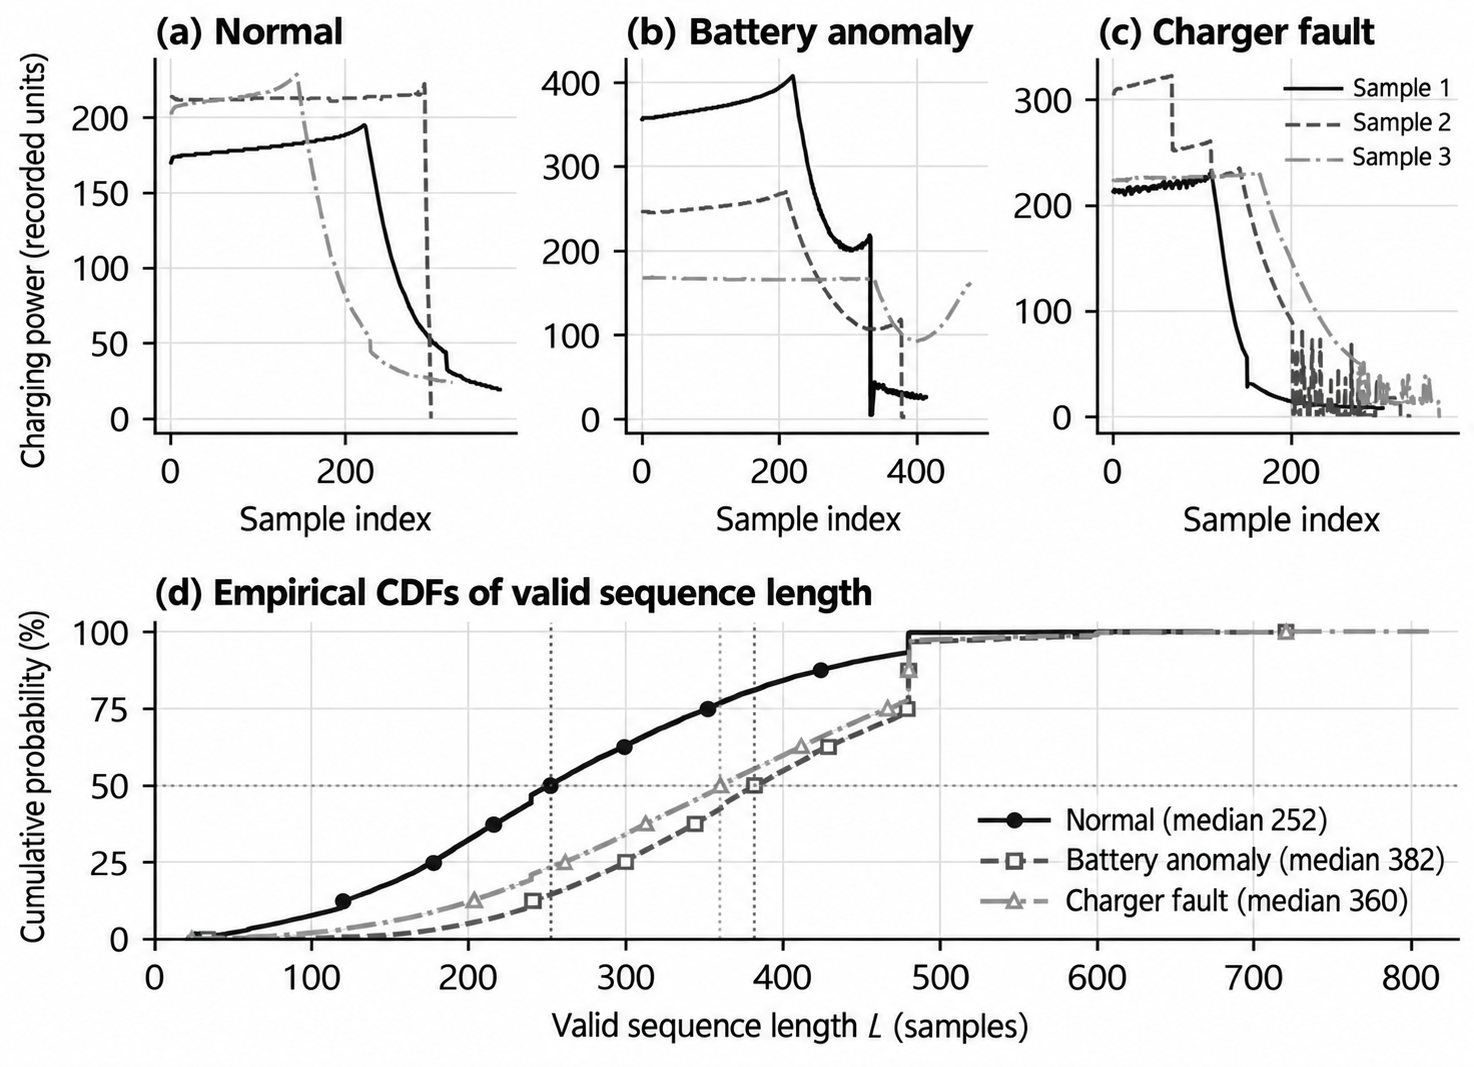
\includegraphics[width=0.92\textwidth]{figures_en/fig1_dataset_overview.png}
\caption{Examples and valid-length distributions in the training set. Panels (a)--(c) show three randomly selected sequences per class using seed 42. Panel (d) shows empirical cumulative distributions and class medians. The sharp rise near 480 samples reflects a common truncation point in the platform records.}
\label{fig:data}
\end{figure}

The median valid lengths are 252, 382, and 360 samples for normal charging, battery anomalies, and charger faults, respectively. A depth-three decision tree trained on length alone obtains 35.76\% test Macro-F1, compared with 17.98\% for the majority-class baseline. Length is therefore a potential shortcut. All sequence models use masks, and section~\ref{sec:fusion} also reports results by length group.

\subsection{Evaluation metrics}\label{sec:metrics}

The class counts are similar but not identical. The primary metric is the unweighted mean of the classwise F1 scores,
\begin{equation}
\mathrm{Macro\mbox{-}F1}=\frac{1}{3}\sum_{c=0}^{2}\frac{2P_cR_c}{P_c+R_c},
\label{eq:macrof1}
\end{equation}
where $P_c$ and $R_c$ are precision and recall for class $c$. Because missing a battery anomaly is the most safety-relevant error, we also report recall for class 1 and its false-positive rate (FPR), defined as the proportion of non-battery-anomaly records predicted as class 1. Average precision is used for single-seed analyses because a precision--recall curve is more informative than an ROC curve for an imbalanced binary evaluation~\cite{saito2015}. Probability quality is measured by expected calibration error (ECE)~\cite{guo2017}. Unless a table states otherwise, all tabulated scores are Macro-F1 values in percent.

\section{Method}\label{sec:method}

\subsection{Overview}

The framework in figure~\ref{fig:framework} has three branches. Branch I sends the original and first-difference sequences through a shared frozen MOMENT-1-large encoder and uses mask-aware pooling. Branch II extracts 60 raw-scale dynamics (DYN) features and classifies them with a histogram gradient-boosting model (HGB). Branch III applies a six-layer causal dilated TCN and masked mean pooling. Each branch produces three class probabilities. Five-fold out-of-fold (OOF) predictions form a nine-dimensional meta-feature for multinomial logistic regression.

\begin{figure}[htbp]
\centering
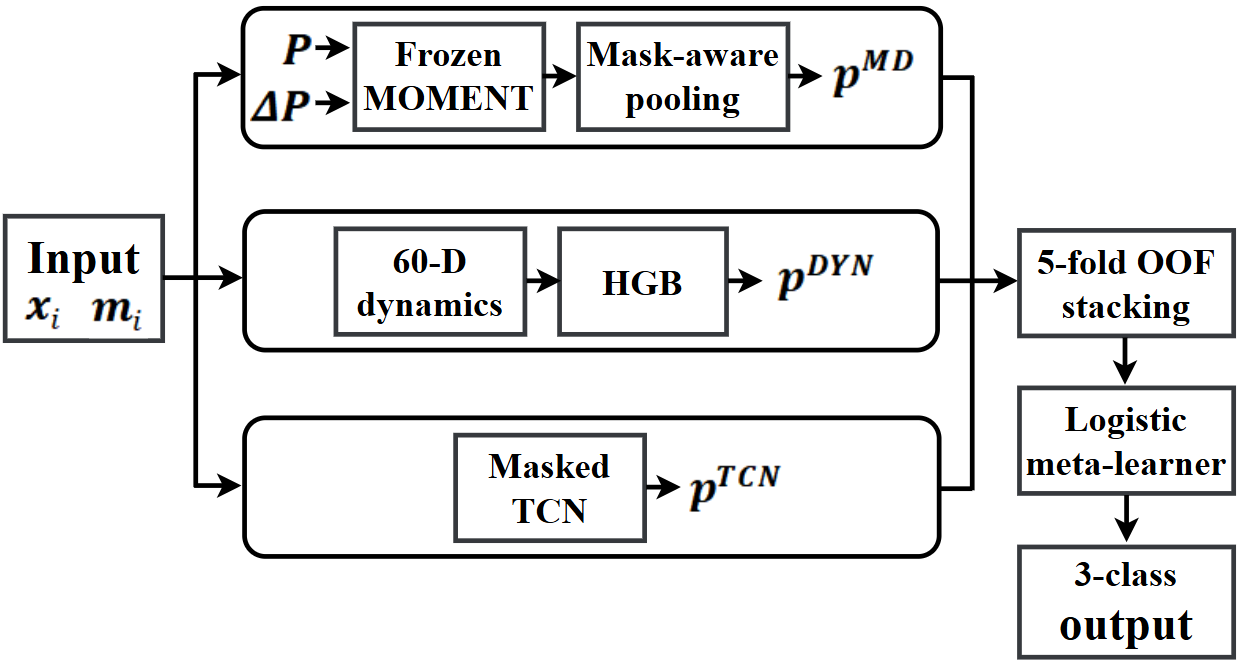
\includegraphics[width=0.78\textwidth]{figures_en/fig2_overall_framework.png}
\caption{Proposed three-branch framework. The original power sequence $P$ and its first difference $\Delta P$ share a frozen MOMENT encoder. The other branches use raw-scale dynamics features and a masked TCN. Five-fold OOF probabilities train the logistic meta-learner.}
\label{fig:framework}
\end{figure}

\subsection{Mask-aware patch pooling}\label{sec:pooling}

MOMENT-1-large uses the T5-large encoder architecture with 24 Transformer layers, a hidden size of 1024, and 16 attention heads. It contains 341.24 million parameters. Similar to PatchTST~\cite{nie2023}, it divides an input of length $T$ into $N=T/P=128$ non-overlapping patches of size $P=8$, producing representations $\bm{h}_{i,1},\ldots,\bm{h}_{i,N}\in\mathbb{R}^{1024}$.

In momentfm 0.1.4, the default classification head passes the input mask into the encoder but averages all patch representations:
\begin{equation}
\bm{z}_i^{\mathrm{default}}=\frac{1}{N}\sum_{n=1}^{N}\bm{h}_{i,n}.
\label{eq:defaultpool}
\end{equation}
For a sequence of length 18, only two of 128 patches are complete; the remaining padded patches dominate the average. By contrast, approximately 78\% of the patches are valid for a sequence of length 800. The degree of representation dilution therefore depends on length.

We define a patch-validity mask
\begin{equation}
\tilde{m}_{i,n}=\prod_{t=(n-1)P+1}^{nP}m_{i,t},\qquad n=1,\ldots,N,
\label{eq:patchmask}
\end{equation}
and pool only complete patches:
\begin{equation}
\bm{z}_i=\frac{\sum_{n=1}^{N}\tilde{m}_{i,n}\bm{h}_{i,n}}{\sum_{n=1}^{N}\tilde{m}_{i,n}}.
\label{eq:maskpool}
\end{equation}
Because $L_i\ge18$, at least two patches are complete and the denominator is nonzero. On fixed synthetic sequences with lengths from 18 to 384, changing the padded length from 512 to 1024 or replacing masked values by random values changes the pooled representation by at most $4.2\times10^{-7}$, which is at the scale of single-precision rounding. This invariance applies to the padded region; external z-score normalization and the model's reversible instance normalization (RevIN)~\cite{kim2022} still use valid observations in an incomplete final patch.

The backbone is frozen, so the representations for all data splits are computed once and cached. Downstream training no longer repeats the 341.24-million-parameter forward pass. One classifier epoch consequently falls from approximately 2~min to approximately 2~s.

\subsection{First-difference dual-stream representation}\label{sec:dual}

Patch encoding and instance normalization favor global shape but can smooth the spikes, slope changes, and plateau transitions that distinguish the classes. Full fine-tuning can recover local information, but it updates all backbone parameters, takes about 3~h per run in our setting, and can overfit at low label budgets. Instead, we expose local change as a second input. Within the valid interval,
\begin{equation}
\Delta x_{i,t}=x_{i,t+1}-x_{i,t},\qquad t=1,\ldots,L_i-1.
\label{eq:diff}
\end{equation}
Slow trends move toward zero, whereas abrupt changes become prominent impulses. The original and difference sequences are z-score normalized separately, passed through the same frozen encoder, and pooled using equation~(\ref{eq:maskpool}). Their concatenation is
\begin{equation}
\bm{z}_i^{\mathrm{MD}}=\left[\bm{z}_i^{P}\,\|\,\bm{z}_i^{\Delta P}\right]\in\mathbb{R}^{2048}.
\label{eq:md}
\end{equation}
An L2-regularized multinomial logistic regression with $C=1.0$ maps this vector to $\bm{p}_i^{\mathrm{MD}}$. The additional cost is one frozen-encoder forward pass per record; no new backbone parameter is trained.

\subsection{Raw-scale dynamics features}\label{sec:dyn}

Per-series z-score normalization and RevIN remove absolute power. This is undesirable when a low-power plateau and a normal constant-power interval have similar normalized shapes. In an early control, a raw-scale TCN obtained 95.99\% test Macro-F1, whereas per-series min--max normalization reduced it to 92.00\%.

The DYN branch therefore extracts 60 features from valid observations at the original scale. Table~\ref{tab:dyn} summarizes the six groups. Fifteen dimensions are standard global statistics; the remaining 45 describe local dynamics, frequency content, and shape. Padding is never used. A fixed HGB classifier uses 400 maximum iterations, learning rate 0.08, 31 maximum leaves, 20 minimum samples per leaf, and L2 regularization 1.0 for every label budget. Feature extraction and HGB training take only seconds on a CPU at the 40\% budget.

For example, the direction-change rate is the fraction of adjacent nonzero differences whose signs reverse; it captures repeated fluctuations. The plateau fraction is the proportion of adjacent samples whose absolute difference is below $10^{-3}$.

\begin{table}[htbp]
\caption{Groups in the 60-dimensional raw-scale dynamics feature vector.}
\label{tab:dyn}
\centering
\begin{tabularx}{\textwidth}{>{\raggedright\arraybackslash}p{3.3cm} c Y >{\raggedright\arraybackslash}p{3.4cm}}
\toprule
Group & Dim. & Representative features & Interpretation \\
\midrule
Amplitude and quantiles & 17 & Mean, standard deviation, extrema, 5th--95th percentiles, coefficient of variation, end/start ratio & Power level and distribution \\
Roughness and turning points & 12 & Absolute-difference statistics, upward fraction, direction-change rate, plateau fraction, longest plateau & Local fluctuation and jump frequency \\
Segment trends & 18 & Global and segment slopes, segment means and deviations, final-minus-initial segment & Constant-power and decay behavior \\
Spectrum and autocorrelation & 7 & Four band-energy ratios, dominant frequency, lag autocorrelation, histogram entropy & Periodicity and complexity \\
Shape & 4 & Maximum drawdown, maximum rise, skewness, kurtosis & Abrupt change and distribution shape \\
Length & 2 & Valid length and fraction of $T$ & Number of valid samples \\
\bottomrule
\end{tabularx}
\end{table}

\subsection{Masked temporal convolutional branch}\label{sec:tcn}

The TCN follows the platform's six-layer causal dilated architecture: kernel size $k=3$, dilations $d_l=2^{l-1}$ for $l=1,\ldots,6$, 128 channels per layer, ReLU activation, and SpatialDropout of 0.3. Its receptive field is
\begin{equation}
R=1+(k-1)\sum_{l=1}^{6}d_l=1+2\times63=127.
\label{eq:rf}
\end{equation}
The original platform network globally averaged the full padded tensor. We replace this operation with
\begin{equation}
\bm{g}_i=\frac{\sum_{t=1}^{T}m_{i,t}\bm{c}_{i,t}}{\sum_{t=1}^{T}m_{i,t}},
\label{eq:tcnpool}
\end{equation}
where $\bm{c}_{i,t}$ is the final convolutional representation. Causality ensures that a valid position does not depend on right padding, and equation~(\ref{eq:tcnpool}) excludes padded outputs. A dense layer and softmax produce $\bm{p}_i^{\mathrm{TCN}}$.

The TCN uses raw-scale inputs and AdamW with learning rate $10^{-3}$, weight decay $10^{-4}$, batch size 32, gradient clipping at 1.0, and a 50-epoch cosine schedule. The epoch-50 endpoint is used in fusion experiments to avoid choosing an epoch on the validation set. Training uses FP32 because FP16 dilated convolutions showed late-epoch overflow on the V100 GPU.

\subsection{Cross-fitted probability stacking}\label{sec:stack}

Training a meta-learner on in-sample predictions would favor overfitted branches. We instead divide each labeled subset $\mathcal{D}$ into five stratified folds. For fold $k$, all three branches train on $\mathcal{D}\setminus\mathcal{D}_k$ and predict $\mathcal{D}_k$. Concatenated OOF probabilities form
\begin{equation}
\bm{u}_i=\left[\bm{p}_i^{\mathrm{TCN}},\bm{p}_i^{\mathrm{DYN}},\bm{p}_i^{\mathrm{MD}}\right]\in[0,1]^9.
\label{eq:meta}
\end{equation}
An L2-regularized multinomial logistic regression estimates
\begin{equation}
P(y_i=c\mid\bm{u}_i)=\frac{\exp(\bm{w}_c^{\top}\bm{u}_i+b_c)}{\sum_{c'=0}^{2}\exp(\bm{w}_{c'}^{\top}\bm{u}_i+b_{c'})}.
\label{eq:softmax}
\end{equation}
Its regularization is selected by an inner three-fold split of the OOF features. Each branch is then retrained on the complete labeled subset for inference. Neither the validation nor the test set enters fitting or hyperparameter selection. The meta-learner has only 30 parameters. When calibrated probabilities are required, a scalar temperature can be fitted on the OOF logits by minimizing negative log likelihood.

\subsection{Noise-augmented training}\label{sec:aug}

The branches above are trained on clean sequences. To test whether sensitivity to acquisition noise (section~\ref{sec:noise}) can be reduced without changing any architecture or hyperparameter, we also train noise-augmented variants, a standard form of time-series data augmentation~\cite{wen2021}. A perturbed copy of each labeled training sequence is generated by adding zero-mean Gaussian noise to valid observations only,
\begin{equation}
\tilde{x}_{i,t}=\max\!\left(0,\;x_{i,t}+\epsilon_{i,t}\right),\qquad \epsilon_{i,t}\sim\mathcal{N}\!\left(0,(\alpha\,\sigma_{\mathrm{rms}})^2\right),\qquad t\le L_i,
\label{eq:aug}
\end{equation}
where $\sigma_{\mathrm{rms}}$ is the root mean square (RMS) of valid observations in the labeled training subset and $\alpha$ is the relative noise level. Masks and padding are unchanged. In the full-system variant, all three branches and the cross-fitted stacker are trained on the clean records together with one noisy copy at $\alpha=0.5\%$; within each outer fold, the model is fitted on both copies of the in-fold records, while the noisy copies of held-out records are excluded. In the DYN-only variant, two noisy copies at $\alpha=0.25\%$ and two at $\alpha=0.5\%$ are added, and the 60 features are recomputed from each copy before HGB training. Evaluation in both cases uses clean or separately perturbed validation records.

\section{Experiments and results}\label{sec:exp}

\subsection{Experimental protocol}\label{sec:protocol}

Label budgets of 1\%, 5\%, 10\%, 20\%, 40\%, and 100\% are sampled stratifiably from the training split, corresponding to 244, 1,227, 2,456, 4,913, 9,827, and 24,569 records. Within a seed, every method uses the same labeled subset and evaluation records. Unless stated otherwise, results are the mean and sample standard deviation over seeds 42, 44, 45, and 46. Method comparisons use paired seed differences and report descriptive 95\% paired $t$ intervals. Exact McNemar tests are used for single-seed error-correction analyses.

The study has three stages. The first stage uses five seeded runs on the same test split to evaluate frozen-MOMENT pooling, adaptation, and pretraining controls. After the test set had been inspected, all further method development and ablation used only the validation set, and the original test partition was not scored again; in the third stage, 753 of its records were reassigned to the sealed hold-out set described below. The four validation splits overlap across seeds and were used repeatedly during development, so paired intervals describe uncertainty within this protocol rather than external generalization.

The third stage limits the effect of this repeated use. A sealed hold-out set of 3,677 records (1,353 normal, 925 battery-anomaly, and 1,399 charger-fault records) is drawn from the 35,099 valid records as 618 whole identifier-prefix clusters, so no cluster is split between the sealed set and the remaining data. The sealed set is identical for all seeds. For each seed, the remaining 31,422 records are re-partitioned into training and validation subsets, and all three branches and the stacker are retrained. The sealed set is not used for fitting, hyperparameter or epoch selection, thresholds, or temperature scaling, and is scored once per seed and label budget. Two qualifications apply. The HGB settings and the TCN architecture were inherited from earlier stages rather than re-selected, and 2,924 sealed records had appeared in earlier training or validation subsets and 753 in the earlier test set. The sealed set therefore guards against selection within this stage, not against every earlier development choice. The noise-augmentation experiments in section~\ref{sec:noise} use validation data only.

Experiments use Python 3.11, PyTorch 2.12.1 with CUDA 12.6, momentfm 0.1.4, and scikit-learn. MOMENT feature extraction and network training use an NVIDIA Tesla V100-PCIE 32~GB. End-to-end latency is measured on an RTX 4080. The unified label-budget reruns, the sealed hold-out experiment, the noise-augmentation experiments, and the model-export measurements use an RTX 5090 host; the export measurements in appendix~\ref{app:export} use PyTorch 2.8.0 with CUDA 12.8.

\subsection{Baselines and initial frozen-model performance}\label{sec:baselines}

Table~\ref{tab:baselines} reports five-seed test results with all training labels. A raw-scale TCN reaches 95.99\% Macro-F1, and a random forest on 15 statistics (F15) reaches 88.89\%. The frozen default MOMENT head yields 69.46\%. Mask-aware pooling alone adds 7.95 percentage points. An RBF-SVM on the corrected representation reaches 85.17\%, unfreezing the final two layers reaches 81.50\%, and full fine-tuning reaches 95.37\% at far higher training cost.

\begin{table}[htbp]
\caption{Test performance with all training labels. Values are mean $\pm$ sample standard deviation over five seeds unless noted.}
\label{tab:baselines}
\centering
\begin{tabularx}{\textwidth}{Y r r r}
\toprule
Method & Trainable parameters & Accuracy (\%) & Macro-F1 (\%) \\
\midrule
Majority class & -- & \pmv{36.94}{0.00} & \pmv{17.98}{0.00} \\
F15 + logistic regression & -- & \pmv{74.13}{0.59} & \pmv{73.75}{0.60} \\
F15 + random forest & -- & \pmv{88.85}{0.23} & \pmv{88.89}{0.23} \\
1D-CNN, per-series z-score & 0.05 M & \pmv{94.29}{1.27} & \pmv{94.38}{1.27} \\
TCN, per-series min--max & 0.22 M & \pmv{91.79}{1.37} & \pmv{92.00}{1.37} \\
TCN, per-series z-score$^{\mathrm{b}}$ & 0.22 M & \pmv{94.92}{1.44} & \pmv{95.02}{1.43} \\
TCN, raw scale & 0.22 M & $\mathbf{95.94\pm0.74}$ & $\mathbf{95.99\pm0.73}$ \\
Frozen MOMENT + linear head, default pooling$^{\mathrm{a}}$ & 3,075 & \pmv{69.53}{0.78} & \pmv{69.46}{0.76} \\
Frozen MOMENT + linear head, masked pooling & 3,075 & \pmv{77.02}{0.88} & \pmv{77.41}{0.89} \\
Frozen MOMENT + RBF-SVM, masked pooling & 0 (backbone) & \pmv{84.77}{1.04} & \pmv{85.17}{1.03} \\
MOMENT, final two layers unfrozen & 25.70 M & \pmv{81.08}{1.13} & \pmv{81.50}{1.06} \\
Fully fine-tuned MOMENT & 341.24 M & \pmv{95.26}{0.41} & \pmv{95.37}{0.39} \\
\bottomrule
\end{tabularx}\\[2pt]
{\footnotesize $^{\mathrm{a}}$ Four seeds completed. The RBF-SVM follows the MOMENT protocol and selects its parameters by five-fold validation on at most 10,000 training records. $^{\mathrm{b}}$ This test-set value coincides numerically with the 10\%-budget validation result of the full model in table~\ref{tab:fusion}; the two come from different protocols.}
\end{table}

Figure~\ref{fig:pooling}(a) summarizes the adaptation sequence. Full fine-tuning approaches the TCN but updates the complete backbone and takes approximately 3~h per run. Frozen feature extraction takes approximately 106~s once, after which downstream models train on a CPU.

\begin{figure}[htbp]
\centering
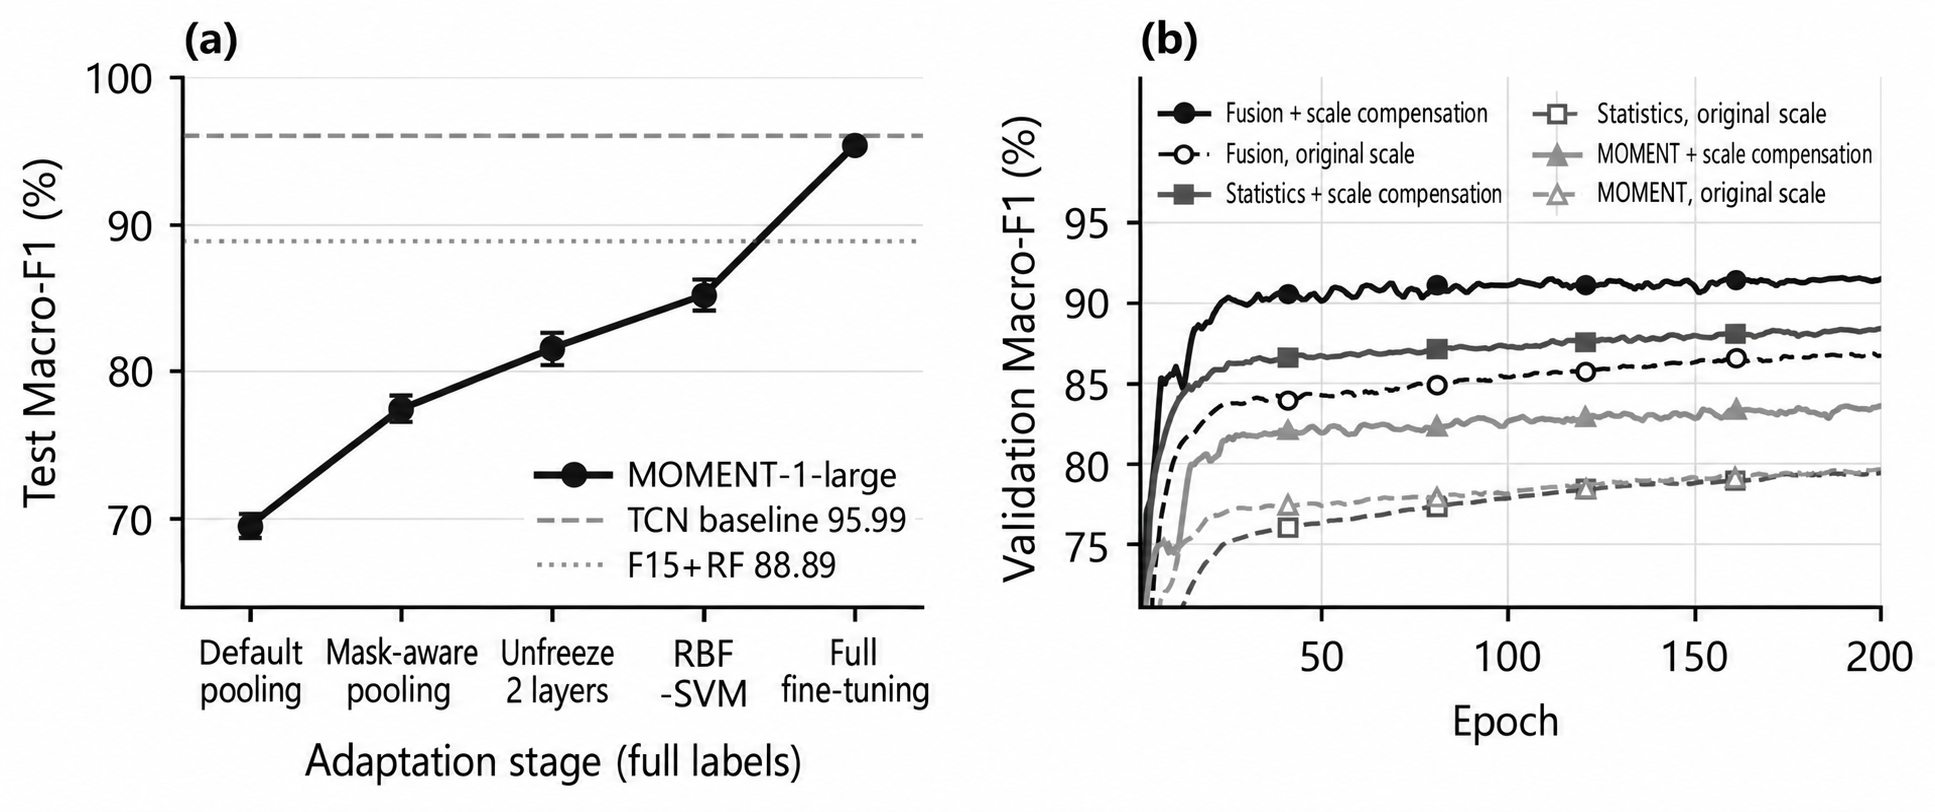
\includegraphics[width=0.96\textwidth]{figures_en/fig3_pooling_and_head_stabilization.png}
\caption{Effects of pooling and downstream optimization. (a) Test Macro-F1 along the MOMENT adaptation sequence. Error bars show seed standard deviations. (b) Validation convergence of frozen-feature heads, with and without fixed input-scale compensation.}
\label{fig:pooling}
\end{figure}

Figure~\ref{fig:pooling}(b) exposes a separate optimization issue. When frozen representations and statistics are concatenated and sent to an MLP head, the initial activation root mean square (RMS) is only 0.024--0.029. Multiplying the input by $\gamma=\sqrt{1039/B}$, where 1039 is the input width of the head and $B$ is the number of active branches, restores an RMS of 0.49--0.55. At epoch 30 this scale correction adds 6.58 percentage points, and the best validation Macro-F1 within 200 epochs rises from 86.94\% to 91.72\%. Across four test seeds, the corrected head reaches $91.52\pm0.38\%$, exceeding an RBF-SVM on the same features by 0.56 points (95\% interval 0.52--0.61). A frozen-model comparison is therefore meaningful only when the downstream head has been adequately optimized.

\subsection{Padding sensitivity and TCN restoration}\label{sec:padding}

The platform's original globally averaged TCN also depends on padding. With weights fixed and valid observations unchanged, increasing total length from 1024 to 1536 changes the largest logit by 418--531 and changes predictions for 100 validation records at the 10\% budget and 33 at the 100\% budget. Masked pooling reduces the measured logit change to zero. Because padding length is usually set by the longest record in a batch, the unmasked model can change its prediction for the same curve when the batch composition changes.

The restored six-layer architecture is also important. An early four-block residual reconstruction with receptive field 61 reaches only $69.23\pm1.61\%$ at 10\% labels. The six-layer network with receptive field 127 reaches $93.68\pm1.93\%$, $97.78\pm0.16\%$, and $98.40\pm0.17\%$ at 10\%, 40\%, and 100\%, respectively (figure~\ref{fig:tcn}(a)). At 1\% and 5\%, however, it falls to $55.51\pm14.66\%$ and $84.03\pm4.57\%$, revealing strong seed sensitivity. Subsequent experiments use this restored masked six-layer TCN as the baseline and ensemble branch.

\begin{figure}[htbp]
\centering
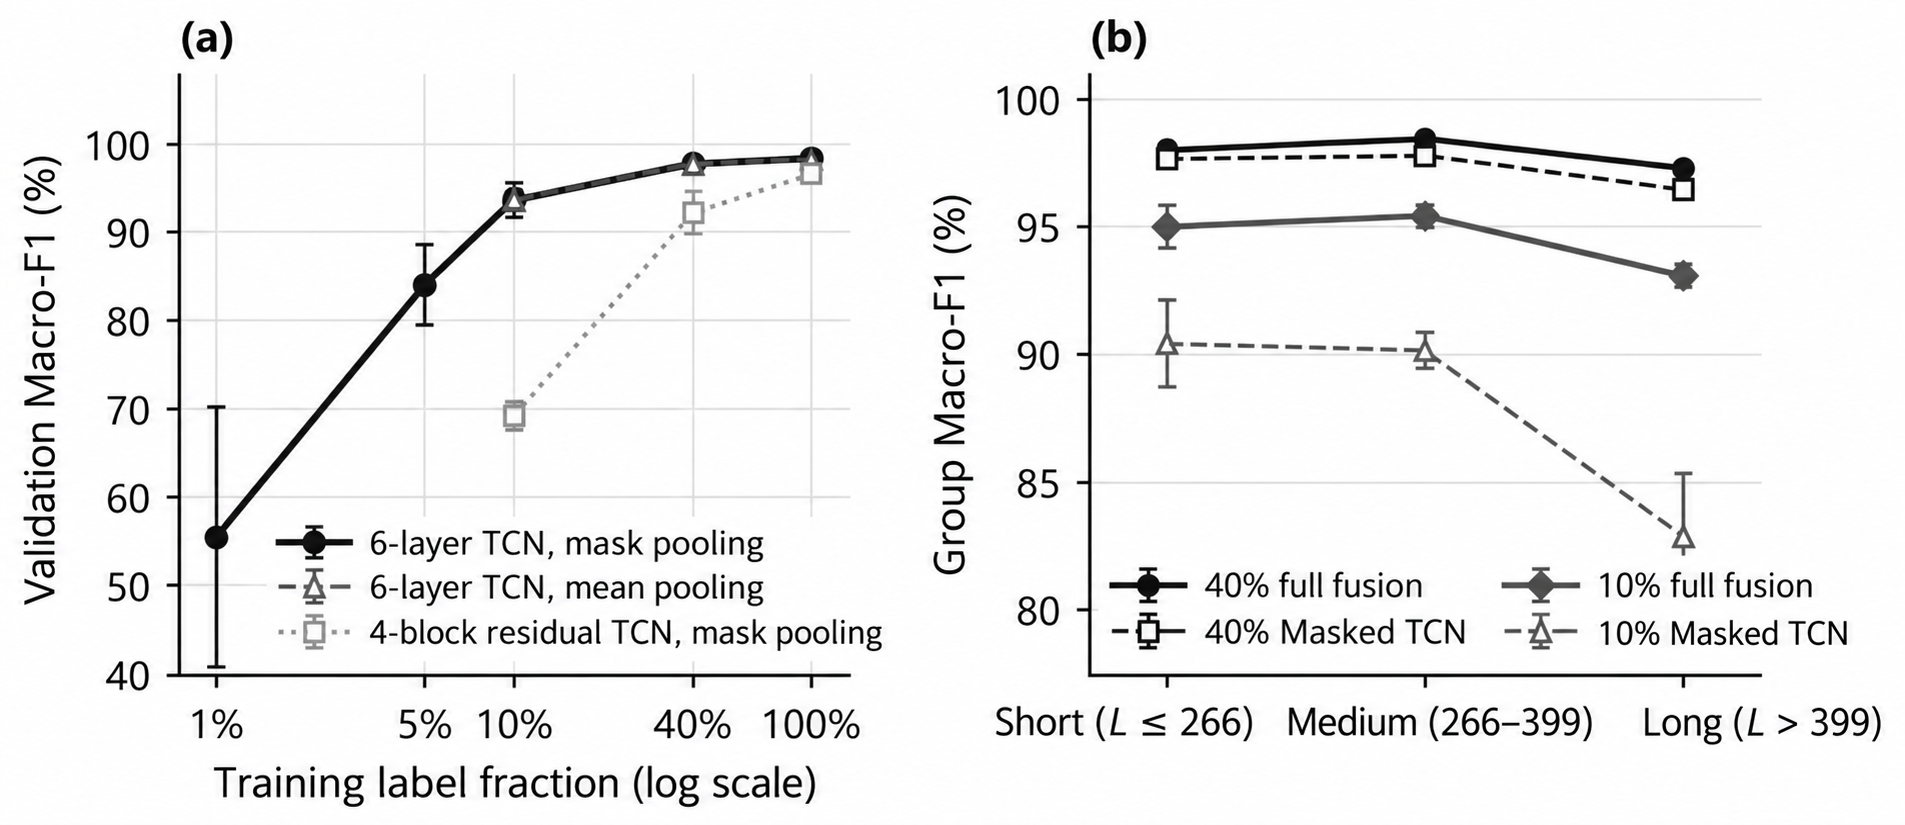
\includegraphics[width=0.96\textwidth]{figures_en/fig4_tcn_and_length_strata.png}
\caption{TCN architecture, pooling, and length-stratified performance. (a) Validation Macro-F1 for three TCN configurations. (b) Performance by seed-specific training-length terciles (approximately 266 and 399 samples). Long sequences exceed the TCN receptive field and show the largest fusion gain at the 10\% label budget.}
\label{fig:tcn}
\end{figure}

\subsection{Difference stream and contribution of pretraining}\label{sec:pretrain}

Figure~\ref{fig:dual}(a) compares frozen MOMENT input streams. The difference stream alone exceeds the original stream. Their concatenation adds 13.38, 10.03, and 9.66 percentage points over the original stream at 1\%, 10\%, and 40\% labels, respectively, with the same direction in all four seeds; at 40\%, the single-branch Macro-F1 rises from 83.91\% to 93.57\%. At 40\%, battery-anomaly recall rises from 89.42\% to 93.36\% and its FPR falls from 3.81\% to 2.56\%. Charger-fault recall rises from 77.87\% to 94.31\%, while its FPR falls from 9.60\% to 3.43\%. Stacking the dual stream with DYN reaches 88.69\% at 1\% labels.

To separate pretraining from encoder capacity, we replace pretrained weights by random initialization while holding the architecture, masks, preprocessing, and downstream classifier fixed. Table~\ref{tab:pretrain} shows that pretrained weights win in every reported condition and seed. For the dual stream, the advantage is 18.81, 9.97, and 6.00 percentage points at 1\%, 10\%, and 40\%, respectively. The benefit increases as labels become scarcer. The difference stream also helps a random encoder, so local differencing and pretrained priors make distinct, additive contributions.

\begin{table}[htbp]
\caption{Same-architecture comparison of pretrained and randomly initialized encoders. Macro-F1 values are percentages.}
\label{tab:pretrain}
\centering
\resizebox{\textwidth}{!}{%
\begin{tabular}{l l r l r r r}
\toprule
Evaluation & Classifier & Labels & Input & Pretrained & Random & Difference (pp) \\
\midrule
Test, five seeds & RBF-SVM & 1\% & Original & \pmv{68.05}{1.59} & \pmv{39.44}{5.00} & $+28.60$ \\
Test, five seeds & RBF-SVM & 5\% & Original & \pmv{77.40}{0.93} & \pmv{54.81}{0.95} & $+22.58$ \\
Test, five seeds & RBF-SVM & 10\% & Original & \pmv{80.77}{0.59} & \pmv{58.76}{1.26} & $+22.01$ \\
Validation, four seeds & Logistic & 1\% & Original & \pmv{68.97}{1.55} & \pmv{46.20}{0.68} & $+22.77$ \\
Validation, four seeds & Logistic & 1\% & Difference & \pmv{80.57}{0.63} & \pmv{64.99}{1.82} & $+15.57$ \\
Validation, four seeds & Logistic & 1\% & Dual & \pmv{83.76}{1.99} & \pmv{64.95}{1.60} & $+18.81$ \\
Validation, four seeds & Logistic & 10\% & Original & \pmv{81.27}{0.35} & \pmv{58.79}{1.13} & $+22.48$ \\
Validation, four seeds & Logistic & 10\% & Difference & \pmv{88.31}{0.84} & \pmv{78.94}{1.07} & $+9.37$ \\
Validation, four seeds & Logistic & 10\% & Dual & \pmv{91.24}{0.57} & \pmv{81.27}{0.91} & $+9.97$ \\
Validation, four seeds & Logistic & 40\% & Original & \pmv{84.02}{0.53} & \pmv{63.45}{1.14} & $+20.57$ \\
Validation, four seeds & Logistic & 40\% & Difference & \pmv{89.20}{0.51} & \pmv{83.03}{1.02} & $+6.17$ \\
Validation, four seeds & Logistic & 40\% & Dual & \pmv{92.77}{0.58} & \pmv{86.77}{0.69} & $+6.00$ \\
\bottomrule
\end{tabular}%
}\\[2pt]
{\footnotesize The validation rows fix the logistic-regression regularization at $C=1.0$, so dual-stream values differ slightly from the single-branch values quoted in the text.}
\end{table}

The three test differences have paired 95\% intervals of 22.24--34.97, 20.89--24.28, and 20.48--23.53 points. On validation data, the dual-stream pretraining advantages at 1\%, 5\%, 10\%, 20\%, and 40\% labels are 18.81, 12.51, 9.97, 7.57, and 6.00 points. Figure~\ref{fig:dual}(b) shows this trend. The 28.60-point test gain of the original-stream RBF-SVM and the 6.00--18.81-point validation gains of the dual stream come from different protocols and are reported separately.

\begin{figure}[htbp]
\centering
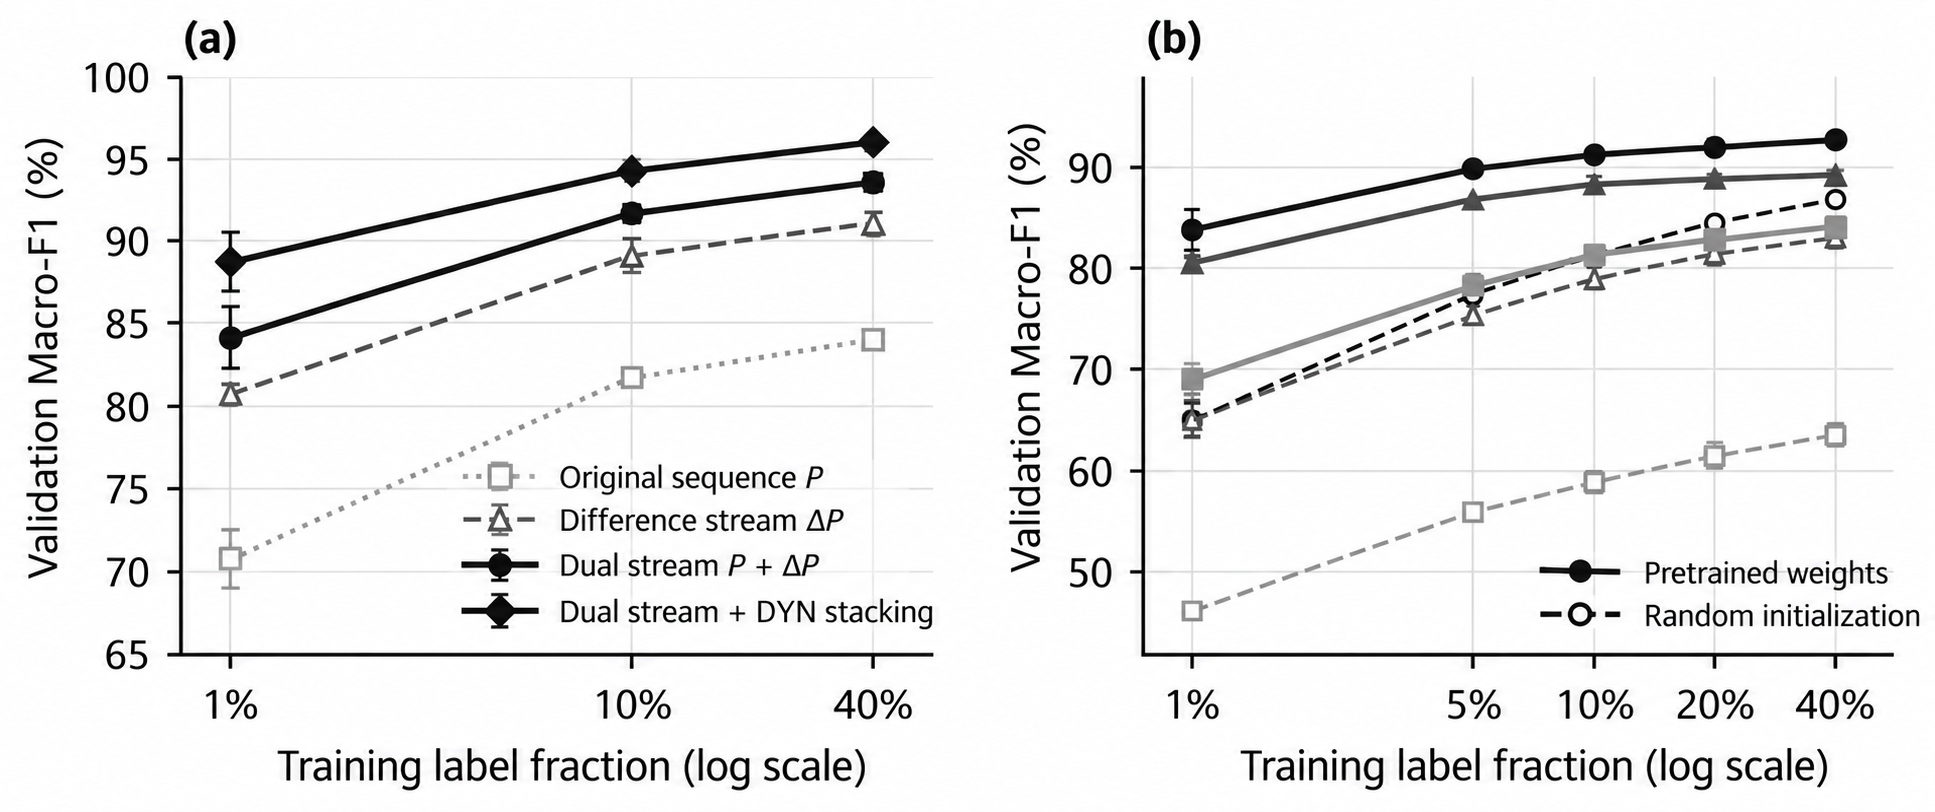
\includegraphics[width=0.96\textwidth]{figures_en/fig5_dual_stream_and_pretraining.png}
\caption{Difference-stream and pretraining effects. (a) Validation Macro-F1 for original, difference, and dual-stream frozen MOMENT representations, with a DYN stack. (b) Same-architecture comparison of pretrained and randomly initialized weights ($C=1.0$).}
\label{fig:dual}
\end{figure}

\subsection{Dynamics features}\label{sec:dynres}

Figure~\ref{fig:dyn}(a) compares the 60 DYN features with the 15 global statistics (F15). DYN is better at every label budget, and HGB is better than RBF-SVM. At 40\% labels, DYN+HGB reaches $95.00\pm0.17\%$, 4.40 points above F15+HGB. At 1\%, it reaches 86.05\%, 8.12 points above F15+HGB and about two points above the frozen dual-stream branch.

\begin{figure}[htbp]
\centering
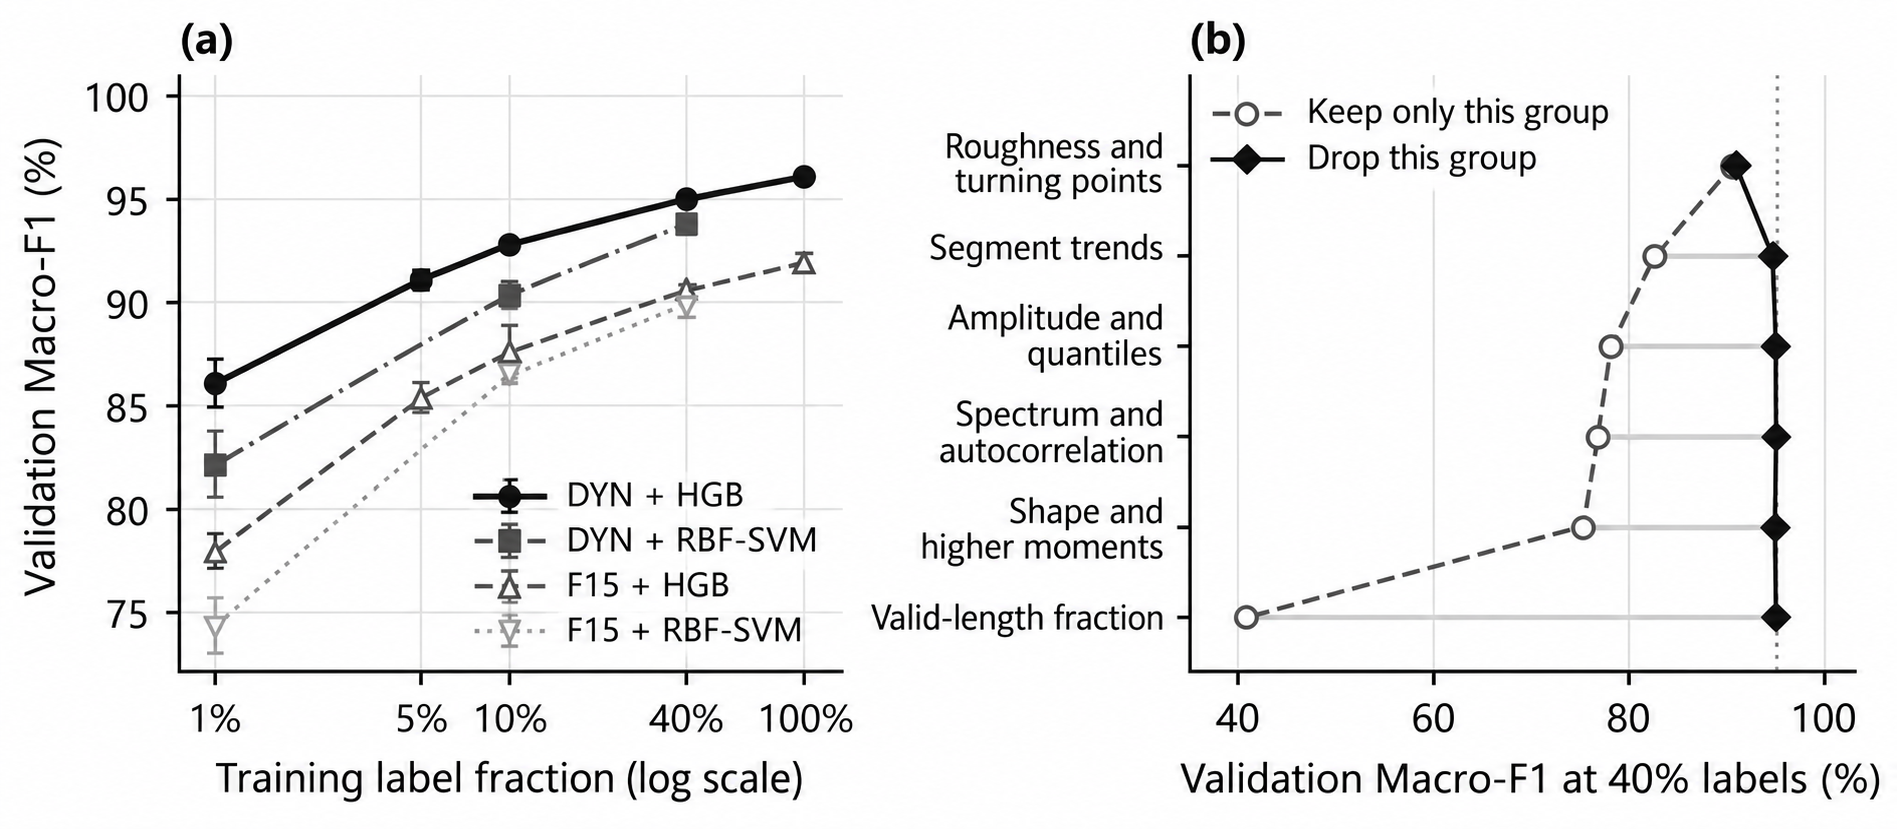
\includegraphics[width=0.96\textwidth]{figures_en/fig6_dyn_feature_ablation.png}
\caption{Raw-scale dynamics features. (a) Label-budget performance of F15 and DYN with HGB and RBF-SVM. (b) Grouped keep-one and drop-one analysis at 40\% labels. The vertical dotted line is the complete DYN result.}
\label{fig:dyn}
\end{figure}

The grouped analysis in figure~\ref{fig:dyn}(b) identifies roughness and turning points as the most important group. Removing it reduces the 40\% result by 4.13 points, whereas using it alone reaches 90.48\%. Segment trends are the next most informative group (82.55\% alone). Removing amplitude, spectrum, or shape individually has little effect, but each group alone still reaches approximately 75--78\%, indicating redundancy. Length alone reaches 40.81\%, confirming that the branch relies mainly on power shape rather than duration.

This redundancy permits a smaller feature set. An exhaustive search over the 63 non-empty group combinations with the HGB settings fixed (appendix~\ref{app:reduction}) shows that the 36 features of the length, trend, roughness, and shape groups are within 0.05 points of the full set at both 10\% and 40\% labels, and that replacing the 60-feature block by this 36-feature block inside the fused model changes Macro-F1 by $+0.19$ and $+0.01$ points, respectively. This conclusion holds for the present groups and classifier; it does not imply that amplitude or spectral features carry no information. All other results retain the 60-feature definition.

\subsection{Fusion and complementarity}\label{sec:fusion}

Table~\ref{tab:fusion} compares eight branch combinations at 10\% and 40\% labels under the same cross-fitted protocol. Full fusion has the highest Macro-F1 at both budgets. At the 10\% budget, the TCN obtains 89.04\% Macro-F1 but already reaches 93.11\% battery-anomaly recall; its charger-fault recall is 77.78\%. Full fusion raises battery-anomaly recall to 95.28\% and lowers the FPR from 2.89\% to 1.87\%; TCN+DYN has marginally higher recall at 95.33\%. At 40\%, full fusion increases battery-anomaly recall from 97.83\% for the TCN to 98.23\% and reduces FPR from 0.77\% to 0.67\%. It exceeds TCN+DYN by only about 0.05 points in recall. Overall accuracy and battery-anomaly recall must therefore be compared separately.

\begin{table}[htbp]
\caption{Validation results of branch combinations under cross-fitted stacking with the joint dual-stream probability block (nine-dimensional meta-feature; four seeds). All logistic regressions use $C=1.0$ and the TCN uses the epoch-50 endpoint.}
\label{tab:fusion}
\centering
\resizebox{\textwidth}{!}{%
\begin{tabular}{l r r r r}
\toprule
Branch combination & Macro-F1, 10\% & Macro-F1, 40\% & Battery recall/FPR, 10\% & Battery recall/FPR, 40\% \\
\midrule
TCN & \pmv{89.04}{0.38} & \pmv{97.53}{0.29} & 93.11 / 2.89 & 97.83 / 0.77 \\
TCN + same-form meta-learner & \pmv{90.71}{0.99} & \pmv{97.65}{0.24} & 93.11 / 2.56 & 97.88 / 0.74 \\
DYN & \pmv{92.81}{0.30} & \pmv{95.00}{0.17} & 92.54 / 2.76 & 95.06 / 2.10 \\
MOMENT/$\Delta P$ & \pmv{91.24}{0.57} & \pmv{92.77}{0.58} & 91.42 / 3.75 & 92.61 / 2.88 \\
DYN + MOMENT/$\Delta P$ & \pmv{94.26}{0.56} & \pmv{96.02}{0.28} & 93.34 / 2.03 & 96.01 / 1.65 \\
TCN + MOMENT/$\Delta P$ & \pmv{93.81}{0.48} & \pmv{97.82}{0.25} & 94.46 / 2.22 & 97.95 / 0.69 \\
TCN + DYN & \pmv{94.26}{0.47} & \pmv{97.93}{0.22} & $\mathbf{95.33}$ / 1.97 & 98.18 / 0.67 \\
\textbf{Full fusion (proposed)} & $\mathbf{95.02\pm0.33}$ & $\mathbf{98.09\pm0.23}$ & 95.28 / $\mathbf{1.87}$ & $\mathbf{98.23}$ / 0.67 \\
\bottomrule
\end{tabular}%
}\\[2pt]
{\footnotesize All values in \%. Recall and FPR refer to the battery-anomaly class (label 1) and are four-seed means.}
\end{table}

Figure~\ref{fig:stack}(a) separates the information gain from the effect of another classifier layer. A meta-learner fed only TCN probabilities adds 1.67 points at 10\% and 0.12 points at 40\%. Full fusion exceeds this same-form control by 4.31 and 0.44 points in all four seeds. Removing TCN from the full model reduces Macro-F1 by 0.76 points at 10\% and 2.07 points at 40\%; removing DYN reduces it by 1.21 and 0.27 points; removing the MOMENT/difference branch reduces it by 0.76 and 0.16 points. TCN contributes most at the higher budget, whereas DYN and MOMENT contribute more when labels are scarce. Adding MOMENT/$\Delta P$ to TCN+DYN is consistently useful at 10\% ($+0.76$ points, four of four seeds, 95\% interval 0.05--1.47); it adds 4.77 points to the TCN alone and 1.45 points to DYN alone. At 40\%, its small mean increment of 0.16 points is positive in three of four seeds and its interval crosses zero.

\begin{figure}[htbp]
\centering
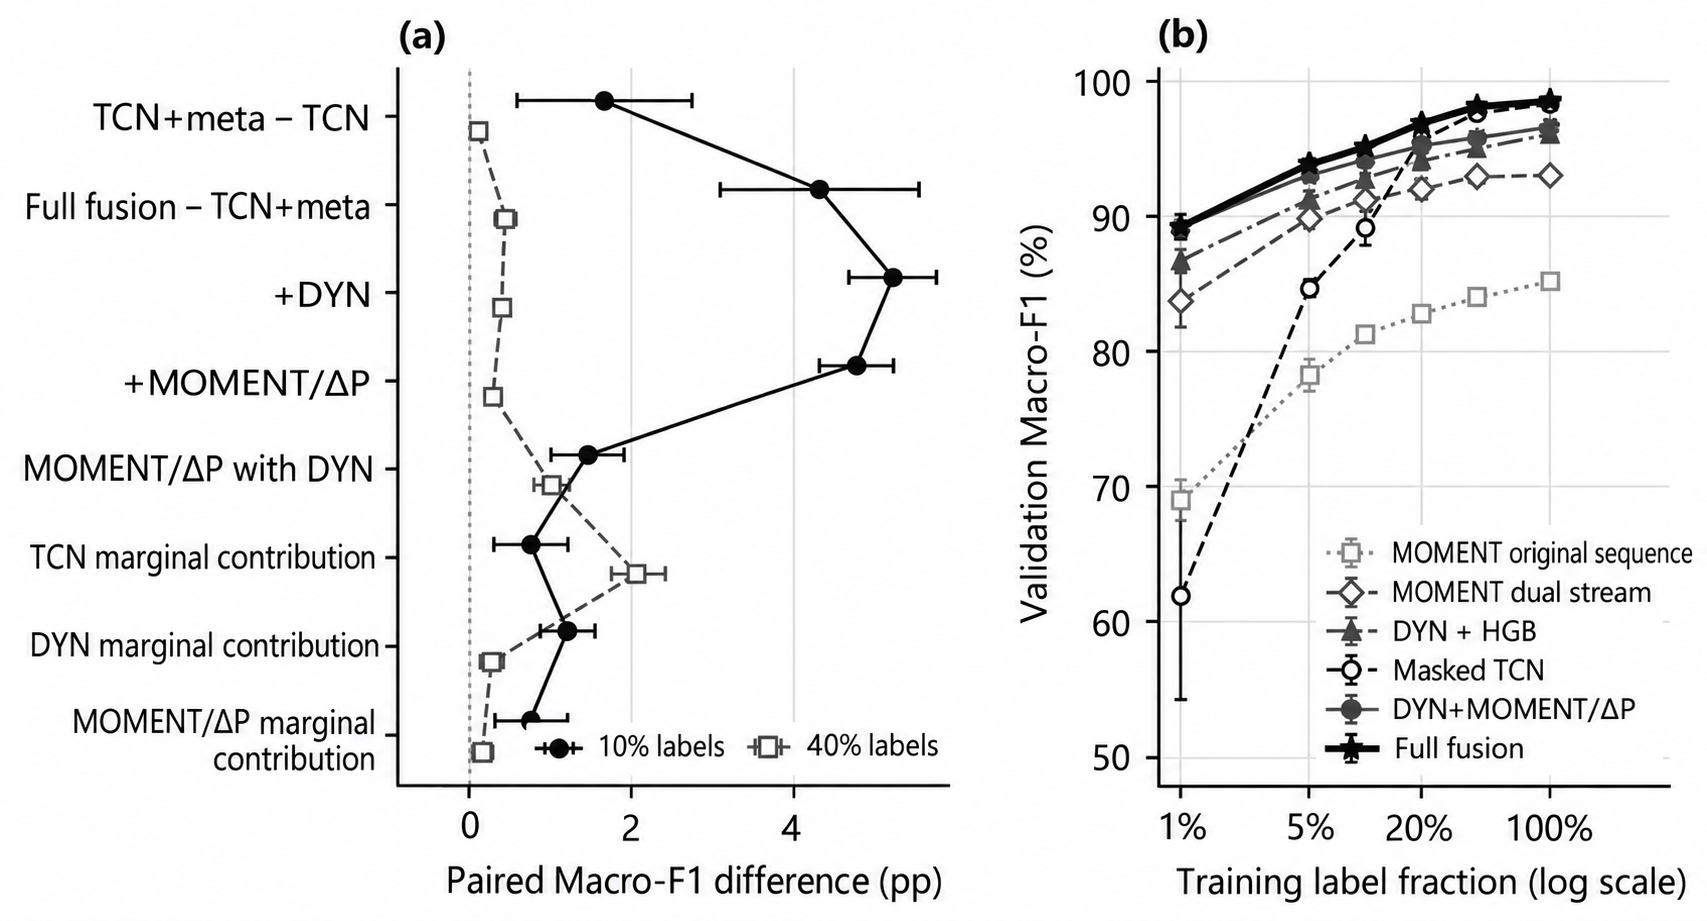
\includegraphics[width=0.96\textwidth]{figures_en/fig7_stacking_ablation_and_low_label.png}
\caption{Complementarity and label-budget effects. (a) Paired branch and same-form meta-learner comparisons at 10\% and 40\% labels. Error bars show seed standard deviations. (b) Validation Macro-F1 under the unified fixed-hyperparameter protocol (table~\ref{tab:budget}). Tick labels at 10\% and 40\% are omitted for legibility; both budgets are plotted.}
\label{fig:stack}
\end{figure}

At 40\%, full fusion corrects 23, 26, 28, and 33 TCN errors across the four seeds while introducing 9, 7, 6, and 7 new errors. Net correction ranges from 14 to 26 records; exact McNemar $p$ values are 0.020, 0.0013, 0.0002, and $4.2\times10^{-5}$. Figure~\ref{fig:tcn}(b) shows the strongest gain for long sequences. At 10\% labels, full fusion raises the long-sequence ($L>399$) Macro-F1 from 82.90\% to 93.07\%, a 10.17-point improvement; at 40\%, it rises from 96.45\% to 97.30\%. In both budgets, the long group gains more than the short and medium groups. Long records exceed the TCN receptive field of 127, whereas global attention directly connects distant patches.

At 40\%, the fused model has an ECE of 0.56\% and an OOF temperature of approximately 1.001, so no rescaling is needed. At 10\%, it is under-confident: mean confidence is 92.21\% while accuracy is 95.01\%, giving an ECE of 3.52\%. OOF temperature scaling ($\tau=0.853$) lowers ECE to 0.94\% and negative log likelihood from 0.1717 to 0.1518. A descriptive validation-set threshold scan for class 1 gives 97.38\% recall at an observed 0.52\% FPR and 98.75\% recall at a 1.04\% FPR for the 40\% model. Because the threshold is selected and evaluated on the same validation data, deployment thresholds must be fixed on a separate calibration set.

\subsection{Label budgets}\label{sec:budget}

Table~\ref{tab:budget} and figure~\ref{fig:stack}(b) summarize the common fixed-hyperparameter label-budget runs. In this protocol, HGB and logistic-regression parameters are not adjusted per budget, the TCN does not select an epoch on validation data, and the meta-feature uses separate probability blocks for the original and difference streams. Full fusion therefore reaches $95.13\pm0.19\%$ at 10\% and $98.14\pm0.01\%$ at 40\% here, compared with $95.02\pm0.33\%$ and $98.09\pm0.23\%$ for the joint-block version in table~\ref{tab:fusion}.

\begin{table}[htbp]
\caption{Validation Macro-F1 (\%) across label budgets under the unified fixed-hyperparameter protocol (four seeds).}
\label{tab:budget}
\centering
\resizebox{\textwidth}{!}{%
\begin{tabular}{l r r r r r r}
\toprule
Method & 1\% & 5\% & 10\% & 20\% & 40\% & 100\% \\
\midrule
F15 + HGB & \pmv{77.91}{0.69} & \pmv{85.34}{0.55} & \pmv{87.75}{1.27} & \pmv{89.30}{0.50} & \pmv{90.57}{0.22} & \pmv{91.87}{0.31} \\
MOMENT, original stream & \pmv{68.97}{1.55} & \pmv{78.21}{1.20} & \pmv{81.24}{0.35} & \pmv{82.79}{0.42} & \pmv{84.00}{0.51} & \pmv{85.12}{0.55} \\
MOMENT, dual stream & \pmv{83.76}{1.99} & \pmv{89.88}{0.72} & \pmv{91.28}{0.56} & \pmv{92.03}{0.75} & \pmv{92.92}{0.62} & \pmv{93.03}{0.31} \\
DYN + HGB & \pmv{86.70}{0.76} & \pmv{91.29}{0.53} & \pmv{92.81}{0.30} & \pmv{94.07}{0.43} & \pmv{95.00}{0.17} & \pmv{96.06}{0.20} \\
Masked TCN & \pmv{61.91}{7.71} & \pmv{84.67}{0.66} & \pmv{89.17}{1.32} & \pmv{95.63}{0.26} & \pmv{97.62}{0.24} & \pmv{98.33}{0.11} \\
TCN + MOMENT/$\Delta P^{\mathrm{a}}$ & \pmv{84.21}{1.94} & \pmv{91.79}{0.39} & \pmv{93.98}{0.44} & \pmv{96.55}{0.04} & \pmv{97.96}{0.18} & -- \\
TCN + DYN$^{\mathrm{b}}$ & \pmv{86.80}{0.93} & \pmv{92.31}{0.89} & \pmv{94.37}{0.38} & \pmv{96.76}{0.18} & \pmv{98.09}{0.09} & $\mathbf{98.54\pm0.18}$ \\
DYN + MOMENT/$\Delta P$ & \pmv{89.12}{0.94} & \pmv{93.03}{0.45} & \pmv{94.18}{0.37} & \pmv{95.25}{0.31} & \pmv{95.80}{0.29} & \pmv{96.58}{0.25} \\
Full fusion & \pmv{89.15}{0.98} & \pmv{93.85}{0.43} & \pmv{95.13}{0.19} & \pmv{96.90}{0.24} & $\mathbf{98.14\pm0.01}$ & \pmv{98.53}{0.16} \\
MultiRocket & $\mathbf{92.52\pm0.34}$ & $\mathbf{95.73\pm0.43}$ & $\mathbf{96.16\pm0.47}$ & $\mathbf{96.92\pm0.29}$ & \pmv{97.25}{0.40} & \pmv{97.67}{0.25} \\
\bottomrule
\end{tabular}%
}\\[2pt]
{\footnotesize $^{\mathrm{a}}$ Uses the joint dual-stream probability block; not run with all labels. $^{\mathrm{b}}$ The value of 98.09\% at 40\% belongs to TCN+DYN in this protocol and is a different system from the full model with the same value in table~\ref{tab:fusion}. The 100\% budget was run as a separate suite with the same settings. All entries are Macro-F1, not classwise recall.}
\end{table}

At 1\%, the TCN averages 61.91\% with substantial seed variation (52.62--71.12\%); selecting the best epoch on validation data raises it only to 64.89\%, and a learning-rate scan over $\{3\times10^{-4},10^{-3},3\times10^{-3}\}$ does not remove the collapse. Adding the MOMENT/difference branch raises TCN+MOMENT/$\Delta P$ to 84.21\% and full fusion to $89.15\pm0.98\%$, 27.24 points above the TCN. Full fusion reaches $93.85\pm0.43\%$ at 5\% and $95.13\pm0.19\%$ at 10\%. Relative to TCN+DYN, its gains at 1\%, 5\%, and 10\% are 2.35, 1.53, and 0.77 points, with descriptive paired intervals of 1.52--3.18, 0.78--2.29, and 0.30--1.23. At 20--40\%, the increment over TCN+DYN shrinks to approximately 0.06--0.14 points and the intervals cross zero. At 40\%, battery-anomaly recall is 98.33\% for full fusion and 98.30\% for TCN+DYN. With all labels, TCN+DYN and full fusion reach 98.54\% and 98.53\%, respectively, so the foundation-model branch has no net benefit at that budget.

MultiRocket, evaluated on the same labeled subsets and validation records, is 3.37, 1.88, and 1.03 points better than full fusion at 1\%, 5\%, and 10\%, ties it at 20\% (96.92\% versus 96.90\%), and is 0.89 and 0.86 points lower at 40\% and 100\%. The proposed model is therefore not uniformly best among time-series classifiers. Section~\ref{sec:selection} discusses when each option should be preferred.

\subsection{Sealed hold-out and cluster-level evaluation}\label{sec:holdout}

Table~\ref{tab:holdout} compares the retrained models on the validation subsets of the third stage and on the sealed hold-out set. At 40\% labels, full fusion scores $97.76\pm0.10\%$ on the sealed set and $97.86\pm0.11\%$ on validation data, with 98.38\% battery-anomaly recall at a 1.02\% FPR. At 10\% labels, the corresponding scores are $94.81\pm0.29\%$ and $94.65\pm0.15\%$. The sealed-set level is 0.3--0.4 points below the earlier 40\% validation estimates of 98.09\% and 98.14\%, which is consistent with the mild optimism expected from repeated use of validation data. These figures come from different partitions and should not be pooled.

\begin{table}[htbp]
\caption{Validation and sealed hold-out results of models retrained without the sealed set (four seeds). The sealed set contains 3,677 records from 618 identifier-prefix clusters and is scored once per seed and budget.}
\label{tab:holdout}
\centering
\begin{tabular}{l l r r r}
\toprule
Labels & Method & Validation & Sealed hold-out & Sealed battery recall/FPR \\
\midrule
\multirow{5}{*}{10\%} & TCN & \pmv{88.55}{1.49} & \pmv{89.41}{1.29} & 93.97 / 2.90 \\
 & DYN & \pmv{92.49}{0.34} & \pmv{92.39}{0.24} & 92.46 / 3.20 \\
 & MOMENT/$\Delta P$ & \pmv{90.81}{0.15} & \pmv{89.92}{0.36} & 91.59 / 4.69 \\
 & TCN + DYN & \pmv{93.73}{0.42} & \pmv{93.96}{0.19} & 94.65 / 2.23 \\
 & Full fusion & \pmv{94.65}{0.15} & $\mathbf{94.81\pm0.29}$ & 95.65 / 2.34 \\
\midrule
\multirow{5}{*}{40\%} & TCN & \pmv{97.41}{0.20} & \pmv{97.32}{0.07} & 98.16 / 1.14 \\
 & DYN & \pmv{94.78}{0.22} & \pmv{94.95}{0.29} & 95.49 / 2.47 \\
 & MOMENT/$\Delta P$ & \pmv{92.18}{0.31} & \pmv{92.04}{0.23} & 93.22 / 3.49 \\
 & TCN + DYN & \pmv{97.84}{0.12} & \pmv{97.68}{0.08} & 98.35 / 1.04 \\
 & Full fusion & \pmv{97.86}{0.11} & $\mathbf{97.76\pm0.10}$ & 98.38 / 1.02 \\
\bottomrule
\end{tabular}\\[2pt]
{\footnotesize Macro-F1, recall, and FPR in \%. The validation column refers to the re-partitioned validation subsets of this experiment, not to tables~\ref{tab:fusion} and \ref{tab:budget}.}
\end{table}

The ranking of the systems is unchanged on the sealed set. Full fusion exceeds TCN+DYN by $0.84\pm0.30$ points at 10\% (four of four seeds) but by only $0.07\pm0.13$ points at 40\% (three of four seeds), which agrees with the shrinking foundation-model increment in sections~\ref{sec:fusion} and \ref{sec:budget}. Relative to its validation score, the TCN rises from 88.55\% to 89.41\% on the sealed set at 10\% and falls from 97.41\% to 97.32\% at 40\%; both changes are within its seed variation.

A leave-cluster-out audit tests whether the stacking layer depends on particular clusters. The validation records of each seed are grouped by identifier prefix and greedily divided into five cluster-disjoint groups; for each group, the meta-learner is re-fitted on the OOF probabilities of the other clusters and evaluated on the held-out group. The branch models are reused, so this audit isolates the stacking layer and does not measure encoder-level transfer. Across the 20 folds, leave-cluster-out stacking reaches $98.14\pm0.52\%$ (lowest fold 96.89\%) at 40\% and $95.18\pm0.81\%$ (lowest fold 93.60\%) at 10\%, compared with $98.12\pm0.16\%$ and $95.14\pm0.37\%$ for in-distribution stacking. The mean is stable, but the spread widens. Per-cluster accuracy of the in-distribution stacker, computed for 71 distinct clusters (121 seed--cluster pairs with 12--23 records each, median 13), falls below 90\% for 11 clusters at 40\% and 20 clusters at 10\%. With so few records per cluster, one or two errors suffice to cross this threshold, so the tail indicates limited robustness across deployment clusters rather than systematic failure of specific clusters.

\subsection{Inference cost}\label{sec:latency}

Table~\ref{tab:latency} reports end-to-end inference on one RTX 4080 for the 40\% models. Timing includes preprocessing, DYN extraction, two frozen-MOMENT passes, the TCN, and all classifier heads, but excludes disk and serving overhead. At batch size 32, full fusion takes 11.13~ms per record, corresponding to about 90 records per second, with 2.49~GB peak GPU memory. At batch size 1, the two MOMENT passes take approximately 33.4~ms (72\%) of the 46.10~ms total, DYN extraction about 2.0~ms, and the TCN about 1.0~ms. The stored FP32 MOMENT backbone is 1,302~MB, compared with 0.9~MB for the TCN, 4.2~MB for HGB, and less than 1~kB for the meta-learner. TCN+DYN is a practical lower-cost operating point when labels are abundant: it is 0.16 points below full fusion at about one fifth of the batched cost.

\begin{table}[htbp]
\caption{End-to-end inference latency on an RTX 4080 for models trained with 40\% of the labels. Values are median milliseconds per record.}
\label{tab:latency}
\centering
\begin{tabular}{l r r r r}
\toprule
Method & Macro-F1 (\%) & Batch 1 & Batch 32 & Batch 128 \\
\midrule
TCN & 97.53 & 0.88 & 0.039 & 0.050 \\
DYN + HGB & 95.00 & 11.43 & 1.99 & 1.83 \\
TCN + DYN & 97.93 & 12.60 & 2.09 & 1.93 \\
Full fusion & 98.09 & 46.10 & 11.13 & 11.42 \\
\bottomrule
\end{tabular}
\end{table}

We also examined whether the TCN tier can be compressed further (appendix~\ref{app:export}). Export to ONNX in FP32 is lossless (maximum logit deviation $\le2.4\times10^{-4}$; TCN and fused Macro-F1 unchanged at 97.53\% and 98.11\%). Static int8 post-training quantization, however, reduces the TCN to 49.34\% and the fused model to 80.08\%, while accelerating batched CPU inference by only about 1.2 times. We hypothesize that the network, which has no normalization layer, produces activations whose dynamic range exceeds a single int8 scale (FP32 logit magnitudes reach 300--1,598 across seeds), but a mixed-precision control has not yet confirmed this explanation.

\subsection{Noise sensitivity and noise-augmented training}\label{sec:noise}

For a noise sensitivity check, zero-mean Gaussian noise is added only to valid observations. Its standard deviation is 0.1\%, 0.25\%, 0.5\%, or 1\% of the training-set valid-observation RMS, which is 192.31 in recorded units, so the levels correspond to approximately 0.19, 0.48, 0.96, and 1.92 recorded units. In the first analysis, all models are trained on clean data without augmentation. As figure~\ref{fig:robust}(a) shows, full fusion remains at 97.72\% under 0.1\% noise and falls to 92.49\% at 0.25\%. At 0.5\%, it falls to 64.00\%, while the TCN remains at 72.00\%. The DYN branch is particularly sensitive because its maximum-rise feature divides by a running minimum; values near zero can amplify a small perturbation. The frozen dual stream degrades more slowly, retaining 85.89\%, 68.23\%, and 46.64\% at 0.25\%, 0.5\%, and 1\% noise. Quantization of the input shows a similar pattern: full fusion reaches 95.44\% at a two-unit step and 64.73\% at a five-unit step.

\begin{figure}[htbp]
\centering
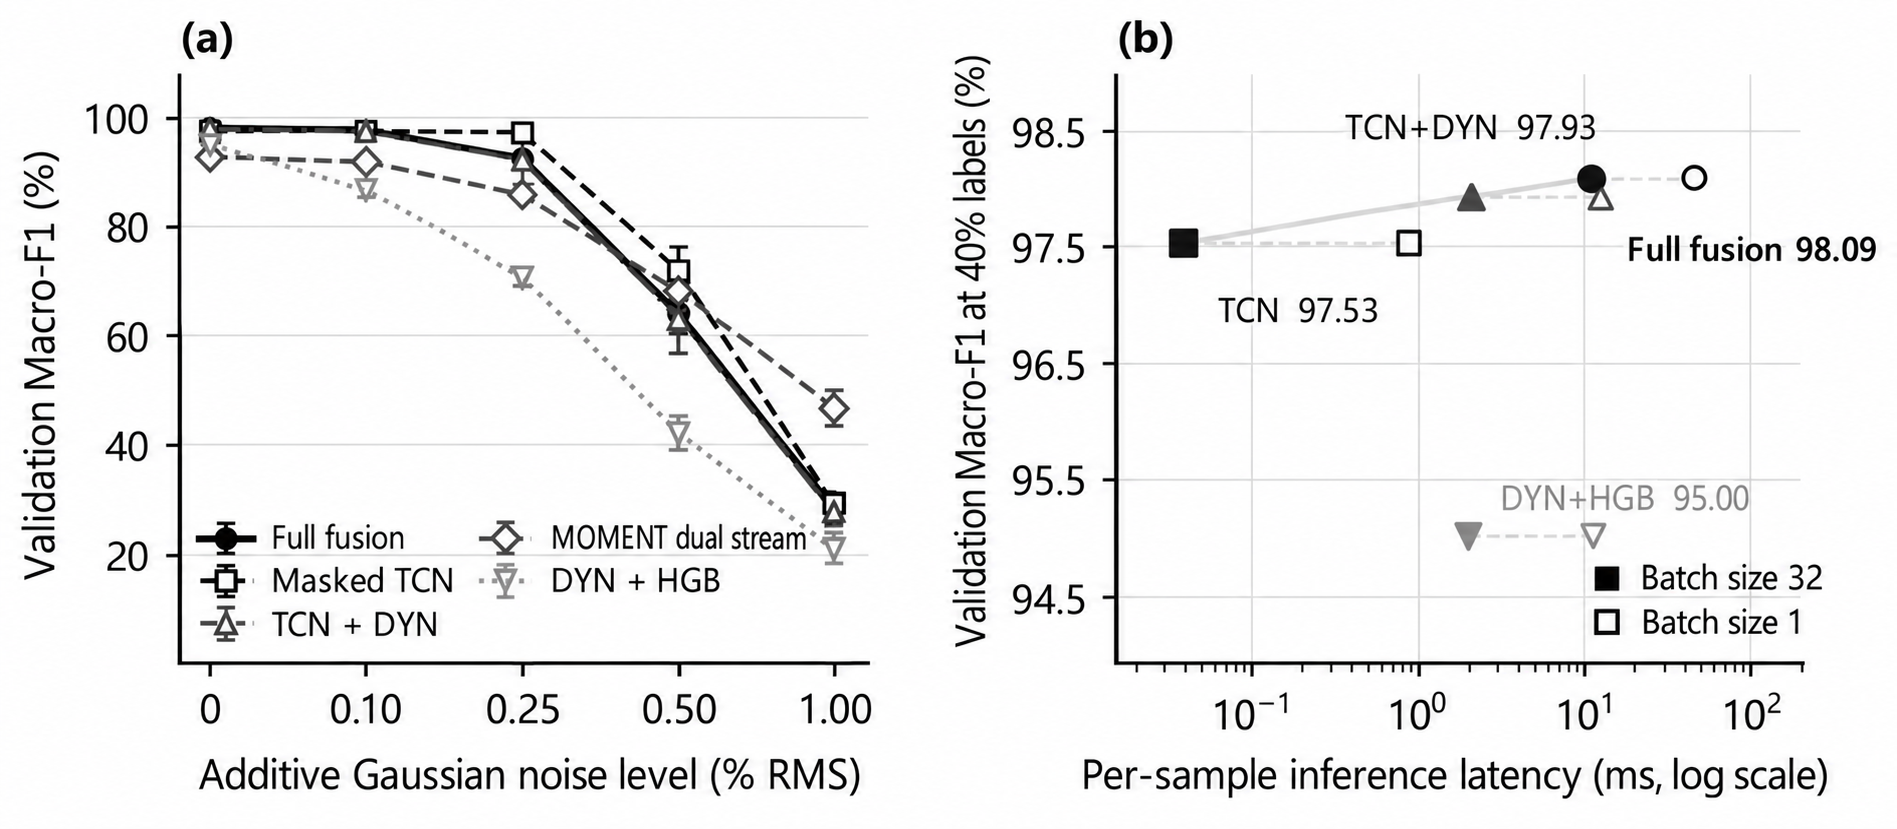
\includegraphics[width=0.96\textwidth]{figures_en/fig8_robustness_and_latency.png}
\caption{Deployment-related analyses at 40\% labels. (a) Validation Macro-F1 after additive Gaussian noise is applied to valid observations; all models are trained on clean data (see table~\ref{tab:noiseaug} for noise-augmented training). (b) Accuracy--latency trade-off for batch sizes 1 and 32 on an RTX 4080.}
\label{fig:robust}
\end{figure}

The risk metrics of clean-trained models change in an unfavorable direction under stronger noise. For full fusion, battery-anomaly recall is 96.71\%, 73.28\%, and 14.10\% at 0.25\%, 0.5\%, and 1\% noise, while its FPR falls to 0.57\%, 0.19\%, and 0.04\%. The lower FPR reflects missed battery anomalies, not improved robustness. Charger-fault FPR simultaneously rises to 11.02\%, 53.21\%, and 92.42\%. At a five-unit quantization step, battery-anomaly recall is 68.01\% with a 0.25\% FPR.

Table~\ref{tab:noiseaug} reports the noise-augmented variants of section~\ref{sec:aug}, with clean-trained and augmented arms scored on the same noise draws. Augmenting only the DYN branch raises its Macro-F1 at 0.5\% noise from 38.21\% to 91.01\% at 10\% labels and from 42.30\% to 93.58\% at 40\% labels (paired gains $+52.79\pm6.39$ and $+51.28\pm2.13$ points, four of four seeds), at a clean-data cost of 1.68 and 0.70 points. This locates most of the clean-trained collapse in the feature branch. Augmenting all three branches removes the clean-data cost: full fusion changes by $+0.74\pm0.21$ points at 10\% (four of four seeds) and $+0.04\pm0.26$ points at 40\% on clean data, while its Macro-F1 at 0.5\% noise rises from 55.39\% to 94.46\% ($+39.07\pm3.85$) and from 64.72\% to 97.47\% ($+32.76\pm1.87$), four of four seeds in both cases. Battery-anomaly recall at 0.5\% noise recovers from approximately 54\% to 95.43\% at 10\% labels and from 73.53\% to 98.65\% at 40\%.

\begin{table}[htbp]
\caption{Validation Macro-F1 (\%) of clean-trained and noise-augmented models under additive Gaussian noise (four seeds). Noise levels are percentages of the valid-observation RMS.}
\label{tab:noiseaug}
\centering
\resizebox{\textwidth}{!}{%
\begin{tabular}{l l l r r r r r}
\toprule
Labels & Model & Training & Clean & 0.1\% & 0.25\% & 0.5\% & 1\% \\
\midrule
\multirow{6}{*}{10\%} & DYN + HGB & Clean & 92.81 & 78.94 & 66.13 & 38.21 & 20.41 \\
 & DYN + HGB & Augmented (0.25\%, 0.5\%) & 91.13 & 89.80 & 90.24 & 91.01 & 44.69 \\
 & Full fusion & Clean & 94.84 & -- & 80.98 & 55.39 & 25.61 \\
 & Full fusion & Augmented (0.5\%) & $\mathbf{95.58}$ & -- & $\mathbf{94.03}$ & $\mathbf{94.46}$ & 45.97 \\
 & MultiRocket & Clean & 96.57 & 94.85 & 88.13 & 62.29 & 30.66 \\
 & MultiRocket & Augmented (0.5\%) & 92.84 & 92.69 & 92.44 & 90.85 & $\mathbf{79.86}$ \\
\midrule
\multirow{5}{*}{40\%} & DYN + HGB & Clean & 95.00 & 86.78 & 71.36 & 42.30 & 21.17 \\
 & DYN + HGB & Augmented (0.25\%, 0.5\%) & 94.30 & 92.70 & 93.21 & 93.58 & 45.60 \\
 & Full fusion & Clean & 97.94 & -- & 92.29 & 64.72 & 28.93 \\
 & Full fusion & Augmented (0.5\%) & $\mathbf{97.98}$ & -- & $\mathbf{97.00}$ & $\mathbf{97.47}$ & $\mathbf{49.30}$ \\
 & MultiRocket & Clean & 97.30 & 95.81 & 89.90 & 64.96 & 33.30 \\
\bottomrule
\end{tabular}%
}\\[2pt]
{\footnotesize For DYN and full fusion, the noise scale is the RMS of the labeled training subset; for MultiRocket it is the RMS of the complete training split (192.14 recorded units). The MultiRocket rows come from a separate run with independent random kernels, so their clean values differ slightly from table~\ref{tab:budget}; a noise-augmented MultiRocket arm was run only at 10\% labels. Clean-trained full fusion was retrained and scored together with its augmented arm on the same noise draws and therefore differs slightly from table~\ref{tab:fusion} and figure~\ref{fig:robust}(a).}
\end{table}

Noise augmentation does not extend beyond the trained level for the proposed system. At 1\% noise, augmented full fusion still falls to 45.97\% and 49.30\%. Augmented MultiRocket, trained with the same single 0.5\% copy, retains 79.86\% at that level, which suggests that the 1\% failure of the proposed system is not solely an information limit of the data, although this comparison is limited to 10\% labels. Within the augmented range, full fusion is more accurate than augmented MultiRocket at 10\% labels (94.46\% versus 90.85\% at 0.5\% noise; 95.58\% versus 92.84\% on clean data), and augmentation costs MultiRocket 3.73 points on clean data. Clean-trained MultiRocket is not more robust than the clean-trained proposed model: it falls from 96.57\% to 62.29\% at 0.5\% noise. These comparisons carry three qualifications: the noise scales are defined on slightly different reference sets, MultiRocket was augmented only at 10\% labels, and both results come from validation data.

\section{Discussion}\label{sec:discussion}

\subsection{Role of the foundation model}

The foundation model requires task-specific adaptation. Without corrected pooling, its frozen representation performs worse than a random forest on simple statistics. Mask-aware pooling removes padding dilution, the first-difference stream restores short changes, and DYN restores raw amplitude. Same-architecture controls show that encoder capacity alone does not explain the final representation: pretrained weights add 6.00--18.81 points to the dual stream across 1--40\% label budgets. The benefit is largest when labels are scarce, and the frozen representation is also more stable than the TCN at 1\% labels (seed standard deviation 1.99 versus 7.71 points).

The branches are complementary rather than interchangeable. MOMENT supplies cross-domain shape priors and global context; DYN supplies interpretable amplitude and roughness; and the TCN learns fine local patterns when enough labels are available. Cross-fitted probabilities let the meta-learner use those differences without training on in-sample confidence. The length-stratified experiments show where the foundation representation adds the most: long sequences at low label budgets ($+10.17$ points for $L>399$ at 10\%). Its benefit also has a clear boundary. The increment over TCN+DYN falls from 2.35 points at 1\% to 0.06--0.14 points at 20--40\% and vanishes with all labels, while the two MOMENT passes account for most of the latency and storage. Above about 20\% labels, TCN+DYN is the more economical choice unless the small remaining gain on long sequences justifies the cost.

\subsection{Alternative adaptation strategies and method selection}\label{sec:selection}

Fully fine-tuning MOMENT reaches 95.37\% with all labels but updates 341.24 million parameters and takes about 3~h per run. The frozen approach needs one feature extraction pass, after which its downstream models train in minutes. These figures come from different label budgets and evaluation stages and should not be treated as a direct accuracy ranking. A rank-eight low-rank adaptation (LoRA)~\cite{hu2022} on the attention projections of all 24 encoder layers adds only 0.45 points over a well-trained frozen fusion head across four seeds while increasing training cost by more than an order of magnitude and requiring backpropagation through the entire encoder. The frozen design was retained on cost-benefit grounds.

MultiRocket remains competitive and is better in the most label-scarce conditions: under the unified protocol it is 1.03--3.37 points more accurate than full fusion at 1--10\% labels, including 1.03 points at 10\%. The crossover near 20\% labels is itself informative: the value of pretrained representations declines as labels increase, whereas random kernels are most valuable when labels are fewest. Together with the noise and cost results, this gives the operating guidance in table~\ref{tab:selection}. The contribution of the present work is therefore an analysis of how to adapt a time-series foundation model to variable-length charging curves and combine it with other representations, not a claim of universal superiority. A four-branch ensemble that adds random-kernel features is a natural extension.

\begin{table}[htbp]
\caption{Operating guidance derived from the validation results. Latency refers to batch size 32.}
\label{tab:selection}
\centering
\begin{tabularx}{\textwidth}{>{\raggedright\arraybackslash}p{4.2cm} Y >{\raggedright\arraybackslash}p{3.3cm}}
\toprule
Condition & Evidence & Preferred option \\
\midrule
1--10\% labels, clean input, CPU-only deployment & MultiRocket exceeds full fusion by 1.03--3.37 points (table~\ref{tab:budget}) & Random-kernel classifier$^{\mathrm{a}}$ \\
10\% labels, noise up to 0.5\% RMS & Augmented full fusion 94.46\% versus augmented MultiRocket 90.85\% at 0.5\% noise (table~\ref{tab:noiseaug}) & Noise-augmented full fusion$^{\mathrm{b}}$ \\
Long records ($L>399$), 10\% labels & Full fusion exceeds the TCN by 10.17 points & Full fusion \\
40\% labels, GPU available & Full fusion 98.14\% versus MultiRocket 97.25\% and TCN+DYN 98.09\% & Full fusion \\
100\% labels & TCN+DYN 98.54\% versus full fusion 98.53\% & TCN + DYN \\
$\ge$40\% labels, latency or memory constrained & TCN+DYN within 0.16 points of full fusion at 2.09 versus 11.13~ms per record & TCN + DYN \\
Noise at 1\% RMS (strongest tested level) & Augmented full fusion $\le$49.30\%; augmented MultiRocket 79.86\% at 10\% labels & Improve acquisition; augmented MultiRocket degrades least$^{\mathrm{b}}$ \\
\bottomrule
\end{tabularx}\\[2pt]
{\footnotesize $^{\mathrm{a}}$ MultiRocket latency was not measured on the same hardware as table~\ref{tab:latency}. $^{\mathrm{b}}$ Validation data only; augmented MultiRocket was tested only at 10\% labels, and its noise scale uses the RMS of the complete training split rather than the labeled subset.}
\end{table}

\subsection{Deployment path}

The measured lower-cost path is the TCN+DYN operating point of table~\ref{tab:latency}, which needs no foundation model at inference. Its TCN can be exported to ONNX without loss and processes about 1,140 records per second on eight CPU threads and about 44,600 records per second on an RTX 5090 at batch size 32 (appendix~\ref{app:export}). Further compression has not succeeded. Static int8 quantization destroys the accuracy of the present TCN, and ONNX Runtime is not faster than PyTorch for this small network. Quantization-aware training~\cite{jacob2018} or architectural changes such as normalization or activation clipping would require new training and are left for future work, as is distillation of the fused model into a single network.

\subsection{Limitations}

The data come from one operating platform and one export. They lack device model, site, calendar time, and sampling-interval metadata, and no public benchmark with the same three-class semantics is available; public electric-vehicle charging and battery datasets differ in signal, granularity, or label definition. Cross-site, cross-period, and cross-device generalization has therefore not been established, and we do not claim state-of-the-art performance on other datasets. The sealed hold-out set reduces selection bias within this study, but it is drawn from the same distribution, overlaps earlier development subsets, and inherits earlier architecture and hyperparameter choices. The leave-cluster-out audit re-fits only the stacking layer, and identifier prefixes are only a proxy for deployment groups. A new external test set is required before deployment.

Noise-augmented training protects the system only up to the trained level of 0.5\% RMS, and some extreme-ratio DYN features remain numerically unstable. The noise model is additive and Gaussian; drift, dropouts, and other acquisition faults were not tested. The 36-feature reduction holds for the present groups and HGB settings, and the int8 failure has not been causally attributed. Finally, the operational labels are coarse. Class 1 denotes a battery anomaly and class 2 a charger fault under the provider's convention, but detailed failure modes and the provider's original label specification were not released. Curves and feature importance establish statistical associations, not battery-health mechanisms.

\section{Conclusion}\label{sec:conclusion}

This study analyzes why a general time-series foundation model transfers poorly to variable-length electric-bicycle charging curves and proposes three targeted corrections. Mask-aware patch pooling raises the frozen linear-probe test Macro-F1 from 69.46\% to 77.41\% and removes dependence on right padding. A first-difference stream adds 9.66--13.38 points to the frozen branch without training the backbone. A 60-dimensional raw-scale dynamics branch restores amplitude information, reaching 95.00\% Macro-F1 by itself at the 40\% budget; 36 of its features suffice without measurable loss. Cross-fitted stacking reaches 95.02\% at 10\% labels and 98.09\% at 40\%, with 98.23\% battery-anomaly recall and a 0.67\% FPR at the latter budget. Under the unified label-budget protocol, it reaches 89.15\% at 1\% labels, 27.24 points above the masked TCN. A retrained model scores 97.76\% on a sealed, cluster-disjoint hold-out set at 40\% labels. Training all branches with noisy copies keeps Macro-F1 at 94.46\% and 97.47\% under 0.5\% RMS noise at 10\% and 40\% labels without reducing clean accuracy.

The additional foundation-model benefit is largest for scarce labels and long records, becomes negligible when all labels are used, and carries substantial latency and storage cost. A random-kernel classifier is more accurate below 20\% labels on clean data. Future work should extend noise robustness beyond the trained level, evaluate independent multi-site data, incorporate random-kernel features into the ensemble, and develop quantization-aware or distilled models for edge deployment.

\appendix

\section{Reduced dynamics feature set}\label{app:reduction}
\setcounter{table}{0}
\renewcommand{\thetable}{A\arabic{table}}

All 63 non-empty combinations of the six DYN groups were evaluated with the HGB settings of each seed and budget fixed. The pre-registered rule selected the best combination with 30--40 features, preferring fewer features when the difference was at most 0.10 points. Table~\ref{tab:reduction} lists the relevant combinations. The 34-feature set without the length group loses 0.38 points at 10\% labels and was not adopted. At the fusion level, the TCN and MOMENT/$\Delta P$ branches were frozen and only the DYN block and meta-learner were re-fitted. Noise-augmented training remains effective with 36 features: at 0.5\% noise it raises DYN Macro-F1 from 35.68\% to 90.78\% at 10\% labels and from 42.60\% to 93.52\% at 40\% labels.

\begin{table}[htbp]
\caption{Validation Macro-F1 (\%) of reduced DYN feature sets (four seeds). $\Delta$ is relative to the 60-feature set.}
\label{tab:reduction}
\centering
\resizebox{\textwidth}{!}{%
\begin{tabular}{l r r r r r r r}
\toprule
 & & \multicolumn{4}{c}{DYN + HGB} & \multicolumn{2}{c}{Full fusion} \\
\cmidrule(lr){3-6}\cmidrule(lr){7-8}
Feature groups & Dim. & 40\% & $\Delta$ & 10\% & $\Delta$ & 40\% & 10\% \\
\midrule
All six groups & 60 & \pmv{95.00}{0.15} & -- & \pmv{92.81}{0.26} & -- & \pmv{98.11}{0.14} & \pmv{95.09}{0.31} \\
Length, trend, roughness, shape & 36 & \pmv{94.98}{0.37} & $-0.03$ & \pmv{92.76}{0.49} & $-0.05$ & \pmv{98.12}{0.18} & \pmv{95.29}{0.38} \\
Trend, roughness, shape & 34 & \pmv{94.95}{0.51} & $-0.06$ & \pmv{92.43}{0.64} & $-0.38$ & -- & -- \\
Trend, roughness, spectrum, shape & 41 & 95.05 & $+0.04$ & 92.82 & $+0.01$ & -- & -- \\
\bottomrule
\end{tabular}%
}\\[2pt]
{\footnotesize The 60-feature fusion baseline differs from table~\ref{tab:fusion} by 0.02--0.07 points because the DYN block and meta-learner were re-fitted.}
\end{table}

\section{TCN export and int8 quantization}\label{app:export}
\setcounter{table}{0}
\renewcommand{\thetable}{B\arabic{table}}

The TCN of each 40\% model (0.22~M parameters) was exported to ONNX (opset 17) with dynamic batch size and separate signal and mask inputs. Static int8 quantization used the QDQ format with unsigned 8-bit activations, signed 8-bit per-channel weights, and 256 training records for calibration. For the fused score, only the TCN probability block was replaced and the meta-learner was re-fitted on the OOF features. Four further configurations (entropy or percentile calibration, symmetric activations, per-tensor weights) gave TCN Macro-F1 of 53.20--58.02\% for seed 42, compared with 97.61\% in FP32. Latencies in table~\ref{tab:export} are medians of 11 repetitions on the RTX 5090 host and depend on the thread count; they are not directly comparable with table~\ref{tab:latency}, which was measured on another machine.

\begin{table}[htbp]
\caption{Accuracy and latency of the exported TCN at 40\% labels (four seeds).}
\label{tab:export}
\centering
\resizebox{\textwidth}{!}{%
\begin{tabular}{l r r r r}
\toprule
Backend & TCN Macro-F1 (\%) & Fused Macro-F1 (\%) & Max.\ logit deviation & Size \\
\midrule
PyTorch FP32 & 97.53 & 98.11 & -- & -- \\
ONNX FP32 & 97.53 & 98.11 & $\le2.4\times10^{-4}$ & 1.0 MB \\
ONNX int8 (static) & 49.34 & 80.08 & 1213.9 & 0.3 MB \\
\midrule
Backend & Threads & Batch & ms per record & Records per second \\
\midrule
PyTorch CUDA FP32 & -- & 1 & 0.22 & 4,604 \\
PyTorch CUDA FP32 & -- & 32 & 0.02 & 44,631 \\
PyTorch CPU FP32 & 8 & 32 & 0.88 & 1,140 \\
ONNX Runtime CPU FP32 & 8 & 32 & 1.23 & 811 \\
ONNX Runtime CPU int8 & 8 & 32 & 0.99 & 1,012 \\
PyTorch CPU FP32 & 1 & 1 & 4.02 & 249 \\
ONNX Runtime CPU int8 & 1 & 1 & 1.20 & 836 \\
\bottomrule
\end{tabular}%
}\\[2pt]
{\footnotesize The fused change from int8 is $-18.03\pm8.49$ points (seeds: $-25.97$, $-7.73$, $-26.85$, $-11.59$).}
\end{table}

\section*{Ethical statement and conflict of interest}
This study uses anonymized device-level charging power sequences and operational status labels. It contains no human participants, human biological material, personally identifying information, or animal experiments; institutional ethics approval was therefore not applicable. The authors declare no conflict of interest.

\funding{This research was funded by the Scientific Research Fund of Hangzhou Dianzi University Information Engineering School, grant number KYP0223008.}

\roles{Zhuotao Qian: methodology, software, formal analysis, investigation, data curation, visualization, and writing--original draft. Chenghua Feng: conceptualization, validation, resources, supervision, and writing--review and editing. Both authors approved the submitted manuscript.}

\data{The charging records are not publicly available because they contain proprietary operational data supplied by an industrial platform. Access requests may be directed to the corresponding author and require approval from the data provider. Code for feature extraction, model training, cross-fitted stacking, and the statistical analyses is available from the corresponding author on reasonable request.}

\section*{References}
\begingroup
\renewcommand{\section}[2]{}
\begin{thebibliography}{99}
\footnotesize
\setlength{\itemsep}{1pt}
\bibitem{feng2018} Feng X, Ouyang M, Liu X, Lu L, Xia Y and He X 2018 Thermal runaway mechanism of lithium ion battery for electric vehicles: a review \textit{Energy Storage Mater.} \textbf{10} 246--267

\bibitem{zhang2023} Zhang J, Wang Y, Jiang B \textit{et al} 2023 Realistic fault detection of Li-ion battery via dynamical deep learning \textit{Nat. Commun.} \textbf{14} 5940

\bibitem{hu2020} Hu X, Zhang K, Liu K, Lin X, Dey S and Onori S 2020 Advanced fault diagnosis for lithium-ion battery systems: a review of fault mechanisms, fault features, and diagnosis procedures \textit{IEEE Ind. Electron. Mag.} \textbf{14} 65--91

\bibitem{park2022} Park S J, Kim W J, Kang B S \textit{et al} 2022 Development of a fault-diagnosis system through the power conversion module of an electric vehicle fast charger \textit{Energies} \textbf{15} 5056

\bibitem{duan2024} Duan Y, Shu S, Zhao Y \textit{et al} 2024 Machine learning-based spatiotemporal fusion method for non-intrusive charging pile fault identification \textit{Front. Electron.} \textbf{5} 1490939

\bibitem{xu2025} Xu Y, Zou Z, Liu Y, Zeng Z, Zhou S and Jin T 2025 Deep learning-based multifeature fusion model for accurate open-circuit fault diagnosis in electric vehicle DC charging piles \textit{IEEE Trans. Transp. Electrif.} \textbf{11} 2243--2254

\bibitem{sun2025} Sun Z, Ye W, Mao Y and Sui Y 2025 A hybrid CNN--LSTM--attention mechanism model for anomaly detection in lithium-ion batteries of electric bicycles \textit{Batteries} \textbf{11} 384

\bibitem{chen2021} Chen W 2021 Research on time-series data classification methods based on deep learning \textit{Master's Thesis} (Wuhan: Huazhong University of Science and Technology) (in Chinese)

\bibitem{xu2026} Xu J, Hu W, Jin D \textit{et al} 2026 Review of time-series data anomaly detection methods \textit{Comput. Sci. Explor.} \textbf{20} 1517--1544 (in Chinese)

\bibitem{fawaz2019} Ismail Fawaz H, Forestier G, Weber J \textit{et al} 2019 Deep learning for time series classification: a review \textit{Data Min. Knowl. Discov.} \textbf{33} 917--963

\bibitem{middlehurst2024} Middlehurst M, Sch\"afer P and Bagnall A 2024 Bake off redux: a review and experimental evaluation of recent time series classification algorithms \textit{Data Min. Knowl. Discov.} \textbf{38} 1958--2031

\bibitem{breiman2001} Breiman L 2001 Random forests \textit{Mach. Learn.} \textbf{45} 5--32

\bibitem{friedman2001} Friedman J H 2001 Greedy function approximation: a gradient boosting machine \textit{Ann. Stat.} \textbf{29} 1189--1232

\bibitem{cortes1995} Cortes C and Vapnik V 1995 Support-vector networks \textit{Mach. Learn.} \textbf{20} 273--297

\bibitem{bai2018} Bai S, Kolter J Z and Koltun V 2018 An empirical evaluation of generic convolutional and recurrent networks for sequence modeling (arXiv:1803.01271)

\bibitem{liu2026} Liu S, Sun J, Qin Y \textit{et al} 2026 Time-series classification based on a multiscale Transformer and morphological convolution \textit{Syst. Eng. Electron.} 1--14 (in Chinese)

\bibitem{yang2026} Yang Y, Hu K, Huang Y \textit{et al} 2026 Classification of VLF/LF lightning electric-field time series using an improved Transformer \textit{High Volt. Eng.} 1--16 (in Chinese)

\bibitem{jiang2026} Jiang T 2026 Research on multivariate time-series forecasting and classification based on an improved Transformer \textit{Master's Thesis} (Huainan: Anhui University of Science and Technology) (in Chinese)

\bibitem{wu2023} Wu H, Hu T, Liu Y \textit{et al} 2023 TimesNet: temporal 2D-variation modeling for general time series analysis \textit{Proc. 11th Int. Conf. on Learning Representations}

\bibitem{dempster2020} Dempster A, Petitjean F and Webb G I 2020 ROCKET: exceptionally fast and accurate time series classification using random convolutional kernels \textit{Data Min. Knowl. Discov.} \textbf{34} 1454--1495

\bibitem{dempster2021} Dempster A, Schmidt D F and Webb G I 2021 MiniRocket: a very fast (almost) deterministic transform for time series classification \textit{Proc. 27th ACM SIGKDD Conf. on Knowledge Discovery and Data Mining} pp 248--257

\bibitem{tan2022} Tan C W, Dempster A, Bergmeir C \textit{et al} 2022 MultiRocket: multiple pooling operators and transformations for fast and effective time series classification (arXiv:2102.00457)

\bibitem{dempster2023} Dempster A, Schmidt D F and Webb G I 2023 Hydra: competing convolutional kernels for fast and accurate time series classification \textit{Data Min. Knowl. Discov.} \textbf{37} 1779--1805

\bibitem{wang2026} Wang S and Yang Z 2026 Transfer randomized neural networks and their learning method for time-series classification \textit{Sci. Technol. Eng.} \textbf{26} 10050--10061 (in Chinese)

\bibitem{yue2022} Yue Z, Wang Y, Duan J \textit{et al} 2022 TS2Vec: towards universal representation of time series \textit{Proc. AAAI Conf. Artif. Intell.} \textbf{36} 8980--8987

\bibitem{goswami2024} Goswami M, Szafer K, Choudhry A \textit{et al} 2024 MOMENT: a family of open time-series foundation models \textit{Proc. 41st Int. Conf. on Machine Learning (PMLR vol 235)} pp 16115--16152

\bibitem{das2024} Das A, Kong W, Sen R \textit{et al} 2024 A decoder-only foundation model for time-series forecasting \textit{Proc. 41st Int. Conf. on Machine Learning (PMLR vol 235)} pp 10148--10167

\bibitem{ansari2024} Ansari A F, Stella L, Turkmen C \textit{et al} 2024 Chronos: learning the language of time series (arXiv:2403.07815)

\bibitem{woo2024} Woo G, Liu C, Kumar A, Xiong C, Savarese S and Sahoo D 2024 Unified training of universal time series forecasting transformers \textit{Proc. 41st Int. Conf. on Machine Learning (PMLR vol 235)} pp 53140--53164

\bibitem{shi2025} Shi X, Wang S, Nie Y \textit{et al} 2025 Time-MoE: billion-scale time series foundation models with mixture of experts \textit{Proc. 13th Int. Conf. on Learning Representations}

\bibitem{shao2026} Shao H, Wang J, Zhang J \textit{et al} 2026 Large-model-driven general fault diagnosis of rotating machinery in multiple scenarios \textit{J. Mech. Eng.} 1--11 (in Chinese)

\bibitem{zhao2026} Zhao X, Li Z, Wang Z \textit{et al} 2026 Deep slope-displacement prediction based on Time-LLM \textit{Hunan Commun. Sci. Technol.} \textbf{52} 29--34 (in Chinese)

\bibitem{yang2026b} Yang J 2026 Time-series forecasting through optimized input representations for large models \textit{Master's Thesis} (Chongqing: Chongqing University of Technology) (in Chinese)

\bibitem{saito2015} Saito T and Rehmsmeier M 2015 The precision-recall plot is more informative than the ROC plot when evaluating binary classifiers on imbalanced datasets \textit{PLoS One} \textbf{10} e0118432

\bibitem{guo2017} Guo C, Pleiss G, Sun Y \textit{et al} 2017 On calibration of modern neural networks \textit{Proc. 34th Int. Conf. on Machine Learning (PMLR vol 70)} pp 1321--1330

\bibitem{nie2023} Nie Y, Nguyen N H, Sinthong P \textit{et al} 2023 A time series is worth 64 words: long-term forecasting with Transformers \textit{Proc. 11th Int. Conf. on Learning Representations}

\bibitem{kim2022} Kim T, Kim J, Tae Y \textit{et al} 2022 Reversible instance normalization for accurate time-series forecasting against distribution shift \textit{Proc. 10th Int. Conf. on Learning Representations}

\bibitem{wen2021} Wen Q, Sun L, Yang F \textit{et al} 2021 Time series data augmentation for deep learning: a survey \textit{Proc. 30th Int. Joint Conf. on Artificial Intelligence} pp 4653--4660

\bibitem{hu2022} Hu E J, Shen Y, Wallis P \textit{et al} 2022 LoRA: low-rank adaptation of large language models \textit{Proc. 10th Int. Conf. on Learning Representations}

\bibitem{jacob2018} Jacob B, Kligys S, Chen B \textit{et al} 2018 Quantization and training of neural networks for efficient integer-arithmetic-only inference \textit{Proc. IEEE Conf. on Computer Vision and Pattern Recognition} pp 2704--2713
\end{thebibliography}
\endgroup

\end{document}
